\documentclass{ctuthesis}

\ctusetup{
    xdoctype = B,
    xfaculty = F3,
    mainlanguage = english,
    titlelanguage = english,
    title-czech = {Vykreslování oblohy a mraků v reálném čase},
    title-english = {Atmosphere and Cloud Rendering in Real-time},
    department-english = {Department of Computer Graphics and Interaction},
    department-czech = {Katedra počítačové grafiky a interakce},
    author = {Matěj Sakmary},
    supervisor = {Ing. Jaroslav Sloup},
    supervisor-address = {Praha 2,\\ Karlovo náměstí 13,\\ E-413},
    month = 5,
    year = 2022,
    specification-file = {zav_prace.pdf},
    keywords-czech = {Volumetrické mraky, Realtime renderování, Atmosféra, Vulkan},
    keywords-english = { Volumetric clouds, Realtime rendering, Atmosphere, Vulkan},
    pkg-listings = true,
    front-specification = false,
}
\ctuprocess
\usepackage{multirow}
\usepackage{caption}
\usepackage{subcaption}
\input{listings-glsl.prf}

\begin{abstract-english}
    This work presents an implementation of the rendering of the volumetric cloud and atmosphere. The implementation aims to combine
    and slightly alter previously published solutions to produce a single unified look.
    Raymarching was used as the main method to render both the atmosphere and clouds. An approach using  
    multiple precomputed Look-up tables (LUTs) proposed by Sébastien Hillaire was used to render the atmosphere.
    This was combined with the option to render volumetric clouds using pre-computed three dimensional texture
    setup storing procedurally generated noise described by Andrew Schneider. The final solution is able to
    render images in high dynamic range before applying post-processing effects and using adaptive luminance
    to transform the image into LDR for presentation.

\end{abstract-english}
    
\begin{abstract-czech}
    Tato práce představuje implementaci renderování volumetrických mraků a atmosféry. Cílem implementace
    bylo zkombinovat a mírně pozměnit dříve publikovaná řešení s cílem vytvořit jednotný vzhled. Metoda
    zvaná Raymarching byla použita pro renderování atmosféry a mraků. Přístup, využívající množství předpočítaných
    Look up tabulek navržen Sébastienem Hillairem, byl použit k renderování atmosféry. Toto 
    bylo zkombinováno s možností vykreslování volumetrických mraků za použití trojrozměrných textur,
    ve kterých je uložen procedurálně generovaný šum, což bylo popsáno Andrew Shneiderem. Konečné řešení 
    je schopno vykreslovat snímky ve vysokém dynamickém rozsahu, na které jsou aplikovány post procesové efekty.
    Tyto snímky jsou poté pomocí adaptivní luminance transformovány do nízkého dynamického rozsahu pro prezentaci
    na obrazovku.
\end{abstract-czech}

\begin{thanks}
    I would like to thank everyone who has supported me during the creation of this work. I would also
    like to thank Ing. Jaroslav Sloup, my supervisor, for offering a lot of valuable advice and 
    guidance throughout the whole process.
\end{thanks}

\begin{declaration}
    I declare that I have created the presented thesis independently and that I have quoted all used sources of
    information in accordance with Methodical instructions about ethical principles for writing academic theses. \\
\end{declaration}

\begin{document}

\maketitle

\chapter{Introduction}
\begin{figure}[h]
    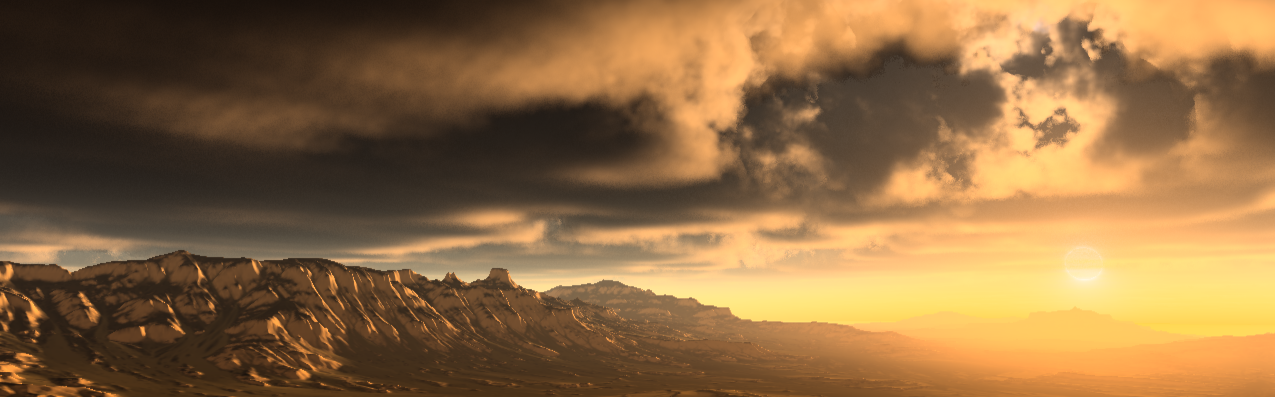
\includegraphics[width=1.0\textwidth]{media/title_image.png}
    \caption[Introduction result image]{Image rendered using our application}
\end{figure}
Having a realistic and believable atmospheric model when rendering dynamic environments in games or other
interactive applications is an important part of creating virtual worlds. The sky, atmosphere, and cloud configuration can 
instantly change the mood of the scene. This is especially important for applications that require
dynamic time of day and weather. Additionally, these effects are also interconnected and affect each other,
making them even harder to simulate. Despite the gradual increase of compute power available in personal 
computers and laptops simulating the complex light interactions producing visual appearance of sky and
clouds is still very difficult. Paired with the constraint of displaying such effects in real time
makes this problem even harder.To avoid these problems, we are forced to adapt number of approximations,
sacrificing a small amount of visual quality but in turn gaining a big reduction in the problem complexity. 

\section{Goals}
The goal of this work was to provide a complete solution to show dynamic clouds and the sky in real time.
To achieve this, we try to combine multiple well-described techniques into a single solution. Additionally,
we wanted to have the option to modify most of the sky and cloud look directly inside of the application
without big delays or freezes. 

Due to the already large scope of our work, we decided that the whole frame-time 
budget will be dedicated to the rendering of desired effects. Our initial aim was to render
previously described effects in 60 frames per second throughout most of the application execution.
Later we decided to lower this value to 30 frames per second in order to produce better looking results.
It is important to note that the application frame rate is highly dependent on the parameterization and
the desired quality of the final image. This means that even though the application frame rate can fall 
below 60 fps, it is still possible to trade some of the visual fidelity for the sake of increased performance.


\section{Previous work}
Now we will provide an overview of previous research that involved rendering of the atmosphere, sky, and clouds.
We will describe multiple possible approaches and reason about their advantages and disadvantages.

The most physically accurate method to render volumetric effects such as sky and clouds is to use 
path tracing. This method sends rays from the camera and follows them as they bounce when hitting 
objects in the scene until they reach a light source. Although using this method produces the best
looking effects, the computational complexity is very high. This is mainly given by the amount of rays
we need to send from the camera to reduce the noise in the final image.

Recently, there have been several promising advances in this field, mainly combining path-tracing with neural networks.
These neural networks serve mainly to denoise the resulting image, reducing the amount of needed rays.
A method was also proposed that uses a neural network specifically to render volumetric clouds~\cite{kallweit2017deep}.
The neural network pre-learns spatial flux distribution and later predicts the radiance function for each 
shading configuration.

\begin{figure}
    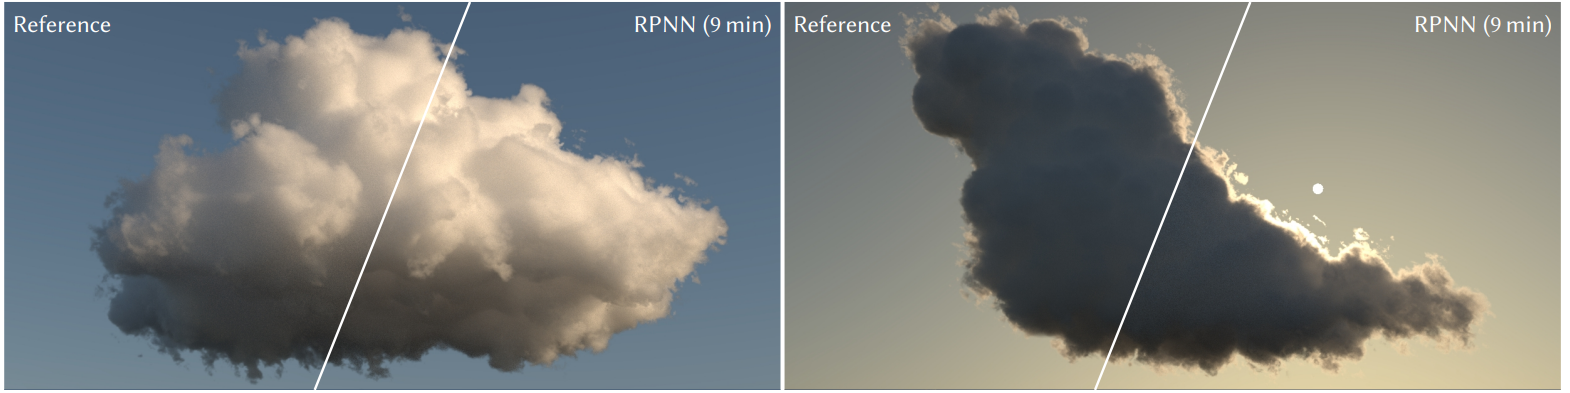
\includegraphics[width=0.9\textwidth]{media/PathTracedCloud.png}
    \caption[Cloud by~\cite{kallweit2017deep}]{Image taken from \cite{kallweit2017deep} showing the cloud rendered using their proposed
        method combining Monte Carlo integration with neural network.}
    \label{fig:pathtraced volumetric cloud}
\end{figure}

Although the proposed improvement reduces the computation time, it is still very difficult to achieve real-time
frame rates while maintaining the desired image quality using these methods. This is why 
they are mainly used in offline rendering or as a ground truth when developing new methods. 

Another approach using fitted mathematical models has also been proposed \\
(\cite{hosek2012analytic}~\cite{wilkie2021fitted}). Methods leveraging this 
principle usually use measured data in order to build a set of parameters used to evaluate the 
sky look. These models tend to be very fast; however, due to the dependence on the data measured
in the real world, these methods fail to provide the option to change the parameters of the atmosphere.
Additionally, when the parameters of the atmosphere are changed, a new model has to be fitted, which is
not possible to do in real time. As the goal of this work is rendering parameterizable atmospheres 
reflecting the conditions present on other planets as well as the ones on Earth, these methods 
did not fit our requirements.

Finally, many methods use ray marching to achieve their results. Offering a good compromise between 
physical accuracy and speed, it is very popular in problems requiring rendering volumetric effects such as clouds, mist,
or atmospheres. Unlike path-tracing, ray marching does not spawn additional rays. Instead, multiple steps are 
taken along a ray, sampling the medium at each step. These medium samples are then used to 
calculate the final look of the ray-marched medium. Because of those reasons, we chose to use ray marching
in our implementation as well. 

\subsection{Sky and atmosphere}

Multiple methods have previously been proposed for rendering physically based atmospheres in real time.
The first ones focused only on single scattering evaluation by ray marching the atmosphere from viewpoint
for each pixel on the screen. Although evaluating only singly scattered light has performance benefits,
it struggles to represent realistic looking atmospheres. This is most visible when trying to represent
more dense atmospheres, where evaluating single scattering only results in dark and unrealistic
scenes. Due to this, methods taking into account multiple scattering were introduced
(\cite{bruneton_neyret_2008}, \cite{yusov2014high}).

Such methods need to rely on precomputing parts of the rendering equation and storing them into 2D,
3D, and 4D tables called Lookup Tables(LUTs) in order to speed up certain parts of the evaluation.
This improves the rendering time significantly because where previously the same evaluation was
repeated tens or hundreds of times, it is now only computed once at the beginning and the results
are then accessed whenever needed, which is much faster. The main drawback of these methods is the
inability to change the atmosphere parameters in real time. Whenever the atmosphere parameters change, all 
of the LUTs used have to be recalculated, which is a very expensive operation. This results in either a long delay 
before seeing the changes caused by time-slicing the operation or worse in the whole application 
freezing until the LUT computations are finished. The second disadvantage is that, because the results
are obtained by ray marching each pixel, the performance is tied to the resolution of the screen.

When trying to solve these problems \cite{hillaire_2020} introduced a new method. The first proposal was a
new method to evaluate multiple scattering inspired by a dual scattering approximation used 
when simulating multiple scattering effects in hair.This reduced the time to precompute LUTs
greatly making it possible to update atmosphere parameters with almost no delay.
The second proposal was to precompute the final sky view and the aerial perspective into fixed-size
latitude/longitude textures, which are later sampled and upscaled. This effectively decouples the
computation complexity from window resolution and introduces additional speed improvements. 

% The method proposed in this work uses the optimizations introduced in \cite{hillaire_2020}.
% However when raymarching the atmosphere Hillaire et al. only assumes linear path of light through
% the atmosphere as well as other approximations which are not strictly physically correct and can be
% improved. The proposed solution is to use approximations described by
% \cite{costa_bock_emmart_hansen_ynnerman_silva_2021}. While this second method does use
% the older and bigger LUT setup, the physical model it proposes is more accurate, approximating
% the path of light through atmosphere not as linear but as elliptical and using more complex
% phase scattering functions. Using such method also makes it possible to simulate atmospheres
% which contain molecules not appearing in earth like atmospheres such as $H_{2}O_{2}$, $NO_{2}$ etc.

\begin{figure}
    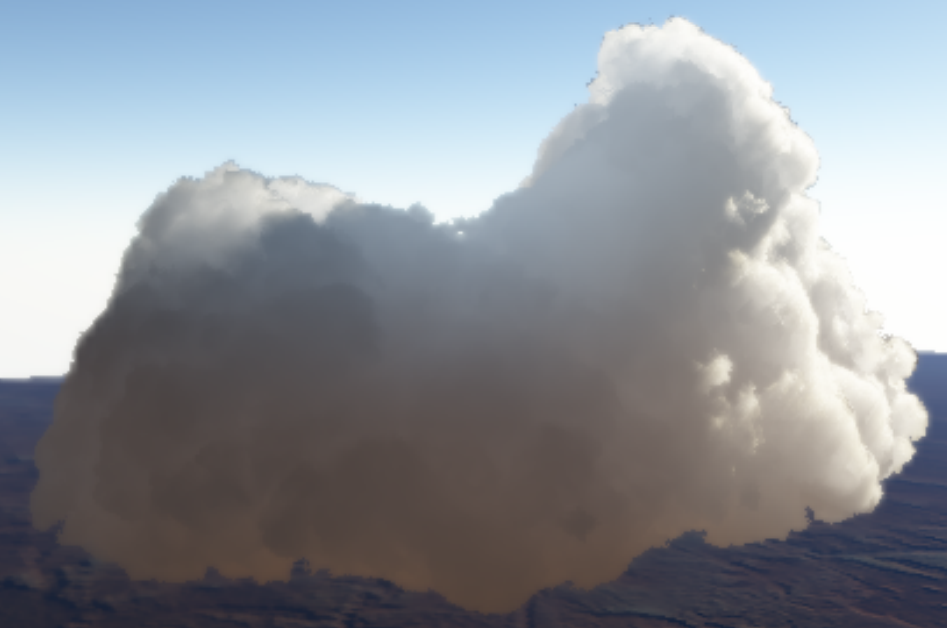
\includegraphics[width=0.8\textwidth]{media/Bouthors_Cloud.png}
    \caption[Cloud by~\cite{bouthors2008interactive}]{Result cloud obtained using method described by~\cite{bouthors2008interactive}}
\end{figure}
\subsection{Clouds}

Many approaches to rendering clouds have been described. Now we will try to summarize the ones that
we found most interesting or relevant to our work. One possible approach to rendering volumetric
clouds was to represent them as volumes of particles. For example, a particle-based rendering method
was previously presented by Yusov~\cite{yusov2014clouds}. The clouds were modeled using copies of
randomly rotated and scaled copies of a single reference particle. The complex optical properties
of this reference particle were precomputed during preprocessing, making this process possible
to use in real-time applications.

\begin{figure}[h]
    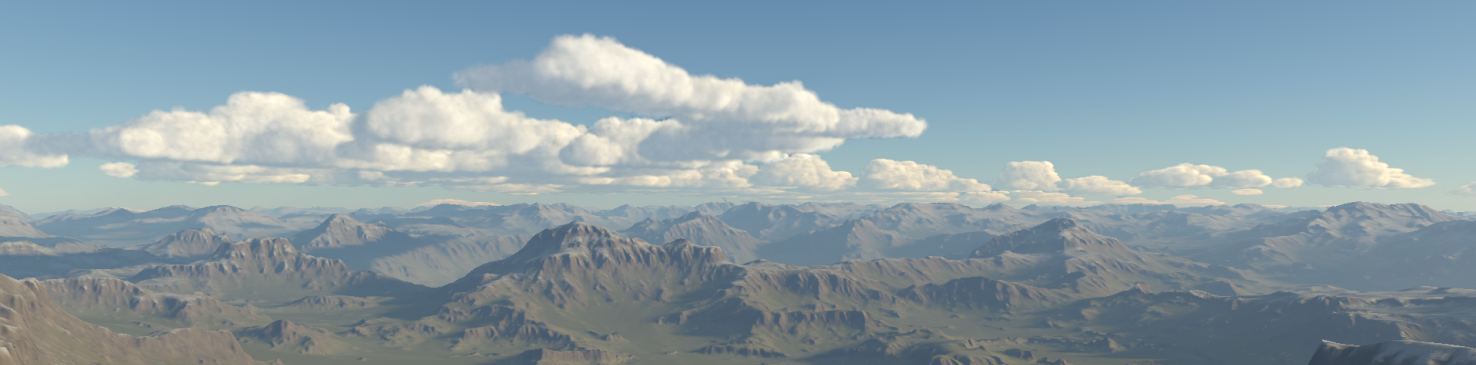
\includegraphics[width=0.9\textwidth]{media/Yusov_clouds.png}
    \caption[Clouds by~\cite{yusov2014clouds}]{Rendered clouds obtained by Yusov et al.~\cite{yusov2014clouds}
        using the reference particle based technique.}
\end{figure}

Another possible technique was presented by Bouthors et al.~\cite{bouthors2008interactive}. By combining
meshes to represent low resolution cloud boundaries together with procedural volumetric hyper-textures
which add the detail under the mesh boundary an efficient cloud representation was achievable. When rendering,
the cloud surface is covered with circular collectors, which are used to evaluate the incoming light. Using
this information along with a set of pre-computed trasfer tables the light is integrated. This produces very
good-looking clouds; however, the cloud representation is not trivial to tweak. This, along with the pretty high
overall complexity of the described method, was the main reason why different, simpler methods were developed.

The most recent work by Schneider~\cite{schneider2015real} uses a fully procedural set of volumetric noise
textures to produce similar results. These noise textures are used to represent changes in density
in a medium caused by clouds. The clouds are then rendered by ray marching the cloud volume and sampling the 
medium. This method also allows us to completely change the overall look of the cloud layer by only tweaking a few
parameters. Additionally, it is possible to simulate dynamic lighting conditions caused, for example, by 
changing the time of day. This was a good fit for our purpose and goals, so we decided to use this method in our
implementation.

\chapter{Physical model}
This section was heavily inspired and contains parts of \cite{petty_2006},\cite{hillaire_2020}, and
\cite{costa_bock_emmart_hansen_ynnerman_silva_2021} that were distilled to contain only parts
relevant to this work. 

\hfill

When electromagnetic radiation (photons of light) travel through the atmosphere, they collide
with molecules the atmosphere consists of. During this collision, part of the energy carried by
the radiation is absorbed, part is reflected (scattered), and part is emitted.

\section{Extinction, Scattering and Absorption Coefficients}
The amount of extinct, scattered and absorbed energy is given by the respective 
\textit{extinction, scattering and absorption coefficients} denoted as 
$\beta_{e}$ ,$\beta_{a}$ and $\beta_{s} $. \textit{Absorption coefficient} is defined as 

\begin{equation}
    \beta_{a} = \frac{4 \pi n_{i}}{\gamma}
\end{equation}

where $\gamma$ is the wavelength of the radiation in vacuum and $n_{i}$ is the complex part of 
\textit{index of refraction}. Thus, this coefficient denotes the rate of energy attenuation per unit of distance at a point x.
Similarly, we define a scattering coefficient. Extinction coefficient 
is then defined by the sum of the absorption and scattering coefficients. 

\begin{equation}
    \beta_{e} = \beta_{a} + \beta_{s} 
\end{equation}

\section{Extinction over a finite path}
\label{extinction over a finite path}

Whenever radiation passes through a medium, its intensity is attenuated exponentially by the 
extinction coefficient represented by the following relationship.
\begin{equation}
    L(\gamma, x) = I(\gamma , 0) \exp(-\beta_{e} x)
\end{equation}
where $\gamma$ is the wavelength of the energy considered. Equation (3) holds under the
assumption that the extinction coefficient is uniform through the atmosphere, which is rarely true. 
To correctly compute attenuation over a path where the extinction coefficient varies, integrating the
coefficient along the entire path of the ray is more suitable. So, to obtain the amount of light that arrives at
the point $x_{2}$ from the point $x_{1}$ given the intensity of light at this starting point and 
\textit{extinction coefficient} $\beta_{e}$ is given by the following relationship.
\begin{equation}
    L(\gamma, x_{2}) = L(\gamma, x_{1}) \exp \bigg[ -\int_{x_{1}}^{x_{2}} \beta_{e}(x) \,dx \bigg]
\end{equation}
Here, the integral quantity inside the brackets is called the optical path 
$\tau$ between the points $x_{1}$ and $x_{2}$
\begin{equation}
    \tau (x_{1},x_{2}) = \int_{x_{1}}^{x_{2}} \beta_{e}(x) \,dx
\end{equation}
By exponentiation of the optical path $\tau$, we get \textit{transmittance} denoted by $T$
between $x_{1}$ and $x_{2}$
\begin{equation}
\label{eq:transmittance}
    T(x_{1},x_{2}) = e^{-\tau(x_{1},x_{2})}
\end{equation}
We can then rewrite the previous equation of light from point $x_{1}$ arriving at point $x_{2}$ as 
\begin{equation}
    L(\gamma ,x_{2}) = T(x_{1}, x_{2})I(\gamma,x_{1})
\end{equation}
Rewriting equations (4) and (7) in a more commonly used form in computer graphics gives us 
\begin{equation}
\label{eq:direct light contribution}
    L(\gamma, x, \overrightarrow{\omega}) = T(x, x_{0}) L(\gamma ,x_{0}, -\overrightarrow{\omega})
\end{equation}
Where $\overrightarrow{\omega}$ is the direction of the ray being evaluated, $x$ is 
the starting point of this ray, and $x_{0}$ is the respective end point of this ray.

\section{Scattering effects of the atmosphere}

So far, the scattering effects of atmosphere particles have only been considered by 
direct attenuation of energy over a path radiation takes through the atmosphere. However,unlike absorption effects, 
when energy is scattered away, it is not converted to another form such
as heat or chemical energy, but instead added back to the atmosphere. This means that the loss 
of energy along one considered path is added along other paths through the atmosphere.

However, the energy scattered away is not uniform in all possible directions. 
To represent this, we use a \textit{scattering phase function} denoted 
$P(\overrightarrow{\omega}',\overrightarrow{\omega})$ where $\overrightarrow{\omega}'$ is the
incoming direction and $\overrightarrow{\omega}$ is the direction of interest (the direction of the ray along which we calculate).

Taking this into account, the scattering formula is denoted as follows.
\begin{equation}
    d L_{scat}(\gamma, x, \overrightarrow{\omega}) = \frac{\beta_{s}}{4 \pi} \int_{4 \pi}
    P(\overrightarrow{\omega}',\overrightarrow{\omega}) L (\gamma, x, \overrightarrow{\omega}')
     \,d\overrightarrow{\omega}' \,ds
\end{equation}

Here, the integral is over $4 \pi$ steradians of the solid angle, and the result is weighed by the
scattering coefficient. To be physically accurate, the concept of energy conservation 
needs to be satisfied (the amount of out-scattered energy cannot be greater than the amount of
incoming energy). This is why the equation is normalized by $4 \pi$. In the later section this 
normalization will be emitted, thus assuming normalized scattering phase function, meaning the following 
must be true.
\begin{equation}
    \int_{4 \pi} P(\overrightarrow{\omega}',\overrightarrow{\omega})\,d\overrightarrow{\omega}' = 1
\end{equation}

When considering an atmosphere, a simplification can be made. Because particles in the
atmosphere are spherical or randomly oriented, the scattering phase function can be 
rewritten to depend only on one parameter $\Theta$ between the original direction and the scattered 
direction. The relationship between those two parameterizations is given as follows.
\begin{equation}
    \cos \Theta = \overrightarrow{\omega}' \cdot \overrightarrow{\omega}
\end{equation}
which simplifies (9) to
\begin{equation}
    d L_{scat}(\gamma, x, \overrightarrow{\omega}) = \int_{4 \pi} \beta_{s}(y) P( cos \Theta) 
    L (\gamma, x, \overrightarrow{\omega}') \,d\overrightarrow{\omega}' \,ds
\end{equation}
Note that $\beta_{s}$ needs to be placed inside of the first integral and is made a function of $y$
since it depends on the distribution of particles inside the atmosphere, which can change with 
position. This will be explained in more detail later.

Applying concepts described in the previous section, the equation for calculating the scattering contribution to a path along a ray with direction $\overrightarrow{\omega}$ arriving at a point $x$ can be computed as follows:

\begin{equation}
\label{eq:scattering contribution equation}
    L_{scat}(\gamma, x, \overrightarrow{\omega}) =  
    \int_{x}^{x_{0}} \beta_{s}(y) T(x,y)  \int_{4 \pi} P( cos \Theta)  
    L (\gamma, y, \overrightarrow{\omega}') \,d\overrightarrow{\omega}' \,dy
\end{equation}

\section{Scattering and extinction effects of clouds}
    Clouds consist of a high concentration of very small water droplets, which generally
    have spherical shape. Because the average radius of water droplets in a cloud is usually around 
    10 $\mu m$, which is much higher than the wavelength of the incoming visible light (380 - 700 $nm$)
    we only consider Mie scattering to occur inside of a cloud (described later in Section~\ref{mie scattering big particles}).

    Most of the concepts described above also apply to clouds. The main difference being the much higher
    scattering and absorption coefficient given by the higher density of particles inside clouds. We use the scattering
    and absorption coefficients measured by~\cite{hess1998optical} together with the computations provided 
    by~\cite{kokhanovsky2004optical}. Please note that these coefficients can also be calculated with the help
    of equations described in Section~\ref{mie scattering big particles}.

    This means that to evaluate the direct contribution of sunlight to the overall luminance can be 
    calculated using Equation~\ref{eq:direct light contribution}. Most of the final white
    look of clouds is caused by the complex scattering effects inside of a cloud. This is due to the high scattering
    coefficient which is why, in contrast to atmospheric computation, multiple scattering effects of clouds
    are much more important. Similarly to the direct light contribution, the scattering contribution can be
    calculated using the previously described equation~\ref{eq:scattering contribution equation}. 
\section{The rendering equation}

If we sum the effects described above by (7) and (12), we get the following form. 
\begin{equation}
\begin{split}
    L(\gamma, x, \overrightarrow{\omega}) &= \underbrace{T(x, x_{0}) L(\gamma ,x_{0}, -\overrightarrow{\omega})}_{direct\ light\ from\ sun}\\ 
    &+\underbrace{ \int_{x}^{x_{0}}  \beta_{s}(y) T(x,y)  \int_{4 \pi} P( cos \Theta)  L (\gamma, y, \overrightarrow{\omega}') \,d\overrightarrow{\omega}' \,dy}_{in-scattered\ light\ along\ the\ ray}
\end{split}
\end{equation}

Because we want to be able to also render effects of opaque objects and thus render
volumetric shadows cast by those objects onto the atmosphere, we also need to add a 
\textit{visibility term} denoted by $V$ introduced by \cite{hillaire_2020}. 
This also enables us to render the effect of a planet as a whole casting a shadow onto the atmosphere,
which can be visible during dusk and sunset as a darker band in the atmosphere just above the
planet's surface. This Visibility coefficient is added to the single scattering evaluation and
is either 0, when the light source is not visible, or 1 when it is visible.

When the currently evaluated ray hits the ground, the effect of radiant energy reflected from 
this point along the ray must also be taken into account. As previously described by 
\cite{bruneton_neyret_2008} and extended by \cite{costa_bock_emmart_hansen_ynnerman_silva_2021},
this energy is calculated by integrating all the energy arriving at the intersection point $s_{0}$
over the hemisphere ($2 \pi$ steradians of solid angle) that is positioned above the tangent 
plane of such a point. This energy is then weighted by the \textit{bidirectional reflectance distribution function (BRDF)} 
denoted as $f(s_{0}, \hat{\Omega}',\hat{\Omega})$ of the planet's surface and the cosine between
the normal at the point $s_{0}$ and the ray incoming direction $\hat{\Omega}'$ 
\cite{costa_bock_emmart_hansen_ynnerman_silva_2021} giving us following formula

\begin{equation}
    R(\gamma, x, \overrightarrow{\omega}) = T(x, x_{0}) \int_{2 \pi} f(x_{0}, \overrightarrow{\omega}',\overrightarrow{\omega}) (n(x_{0}) \cdot \overrightarrow{\omega}') L(\gamma, x_{0},\overrightarrow{\omega}')
\end{equation}

Finally, adding all of this together results in a full rendering equation formula. 

\begin{equation}
\begin{split}
\label{eq:complete rendering equation}
    L_{tot}(\gamma, x, \overrightarrow{\omega}) & = \underbrace{T(x, x_{0}) L(\gamma ,x_{0}, -\overrightarrow{\omega})}_{direct\ light\ from\ sun} \\
    & +\underbrace{T(x, x_{0}) \int_{2 \pi} f(x_{0}, \overrightarrow{\omega}',\overrightarrow{\omega}) (n(x_{0}) \cdot \overrightarrow{\omega}') L(\gamma, x_{0},\overrightarrow{\omega}')}_{light\ reflected\ from\ surface} \\
    & + \underbrace{ \int_{x}^{x_{0}} \beta_{s}(y) T(x,y)  \int_{4 \pi} P( cos \Theta)  L (\gamma, y, \overrightarrow{\omega}') \,d\overrightarrow{\omega}' \,dy}_{in-scattered\ light\ along\ the\ ray}
    \end{split}
\end{equation}

\hfill

\section{Multiple scattering approximation}\label{multiscatt approx}

As described above, calculating only single scattering of light is not sufficient for realistic results.
This is because the scattering of light inside an atmosphere occurs multiple times, so only 
considering a single scatter results in a big loss of calculated energy. When calculating multiple
scattering model proposed by~\cite{costa_bock_emmart_hansen_ynnerman_silva_2021}
and~\cite{bruneton_neyret_2008} uses an iterative approach which can be mathematically denoted as follows:
\begin{equation}
\begin{split}
    L & = L_{0} + (R + S)[L_{0}] + (R + S)[(R + S)[L_{0}]] + \dots \\
    & = L_{0} + L_{1} + L_{2} + \cdots = L_{0} + L_{*}
\end{split}
\end{equation}
where $L_{0}$ is the attenuated direct sunlight that reaches the considered point. 
The big disadvantage of this model is the high computational cost. This quickly becomes a problem 
for denser atmospheres, where multiple scattering of order up to 40 and more has to be evaluated.
The solution to this proposed in \cite{hillaire_2020} is also used in this work. 

The overall smooth distribution of participating media in the atmosphere allows the assumption
that the energy reaching a single point in space is the same for all points within a large area
around it for scattering orders greater than 2. Because of this, the multiple scattering
evaluation can be simplified.

First, second-order scattering is evaluated according to the methods described previously.
\begin{equation}
    L_{2^{nd}order} = \int_{4 \pi} L_{tot}(\gamma, x, -\overrightarrow{\omega}) P(cos \Theta)
\end{equation}
However, instead of integrating luminance, a unitless placeholder factor is used $L_{I}$.
The reason why this is done will be explained later.

\begin{figure}
    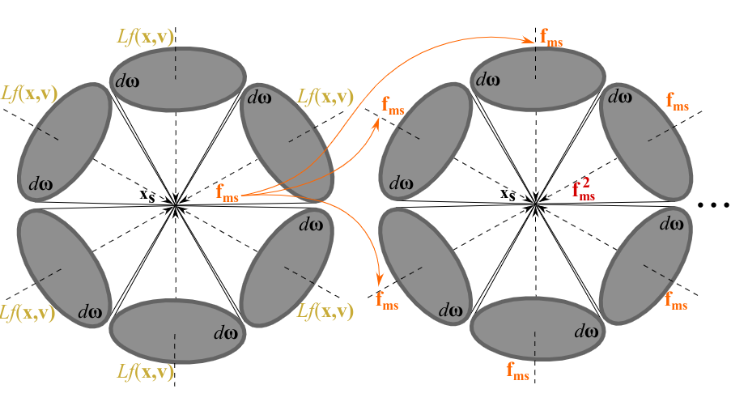
\includegraphics[width=0.9\textwidth]{media/Hillaire_multiscattering.png}
    \caption[$F_{ms}$ and $f_{ms}$ by~\cite{hillaire_2020}]{Image provided by~\cite{hillaire_2020} showing how the
         $F_{ms}$ is computed by using$f_{ms}$.}
\end{figure}

Secondly also untiless factor of \textit{$f_{ms}$} representing the transfer of energy 
that would occur from the area around and aimed towards considered point is calculated by 
\begin{equation}
\label{fms definition}
    f_{ms} = \int_{4 \pi} L_{f}(\gamma, x, -\overrightarrow{\omega}) P(cos \Theta) \,d\overrightarrow{\omega} \\
\end{equation} 
\begin{equation}
\label{Lf definition}
    L_{f}(\gamma, x, -\overrightarrow{\omega}) = \int_{x}^{x_{0}} \beta_{s}(y) T(x,y) 1 \,dy
\end{equation}
Because $f_{ms}$ is in the range between 0 and 1 and given the previous assumption about the 
amount of energy reaching a point for scattering orders greater than two, the infinite multiple
 scattering energy contribution can be approximated by
\begin{equation}
    F_{ms} = 1 + f_{ms} + f_{ms}^{2} + f_{ms}^{3} + \dots
\end{equation}
Given that the value of $f$ lies in the interval [0,1], equation (21) can be solved analytically. 
\begin{equation}
    F_{ms} = \frac{1}{1-f_{ms}}
\end{equation}
Because the placeholder unitless factor was used when calculating the second order of the in-scattered
energy, the total contribution of a directional light with an infinite number of scattering orders
can be evaluated as
\begin{equation}
\label{transfer factor equation}
    \Psi_{ms} = L_{2^{nd}order}F_{ms}
\end{equation}
Finally, Equation (13) should now be modified to give the final form.
\begin{equation}
    L_{scat}(\gamma, x, \overrightarrow{\omega}) = \int_{x}^{x_{0}} (\beta_{s}(y) T(x,y) P(cos \Theta) +  \Psi_{ms})L (\gamma, y, \overrightarrow{\omega}') \,dy
\end{equation}
where $\overrightarrow{\omega}'$ is the direction from the current position $y$ 
to the considered light source.

\section{Physical properties of particles inside atmosphere}
As already mentioned, incoming light in form of electromagnetic radiation collides with particles that make up the atmosphere. The properties of those collisions depend on the wavelength of the incoming radiation, but they also depend on the size of the particle considered. When considering the visible wavelength band (440nm - 680nm), which is the only band in which this work is interested, the scattering effects can be described by two underlying theories, Mie and Rayleigh Scattering.
    
\subsection{Scattering and absorption effects of molecules and atoms}
When considering small particles (that is, particles much smaller than the wavelength of 
the incident radiation $r_{particle} \ll \gamma_{incident\ radiation}$) Rayleigh 
scattering theory is used. Rayleigh scattering phase function is used to approximate 
the angular distribution of the outscattered radiation. The more complicated model proposed by
\cite{costa_bock_emmart_hansen_ynnerman_silva_2021}, which takes into account the anisotropy 
of the atmosphere molecules, is used.

\begin{equation}
    P_{R}(\theta) = 0.7629(1+0.932 \cdot cos^{2}(\theta)) \cdot \frac{1}{4 \pi}
\end{equation}

Note that normalization by 1 over 4 pi is included, as mentioned above. 
For the scattering coefficient, once again the one proposed by 
\cite{costa_bock_emmart_hansen_ynnerman_silva_2021} is used. 
\begin{equation}
    \beta^{scat}_{R}(h, \gamma) = \frac{8 \pi^{3}(n(\gamma)^{2} - 1)^{2}}{3N\gamma^{4}} \cdot e^{-\frac{h}{H_{R}}}\ [m^{-1}]
\end{equation}

Here, $n(\gamma)$ and $N$ are the refractive index of the medium (whose imaginary part was also used in Eq. (1) when describing the absorption index $\beta_{a}$) and the molecular density at sea level, respectively.
Also, note the term $e^{-\frac{h}{H_{R}}}$ that describes the variation of atmospheric density according to height $h$ and scale height $H_{R}$. The change in the density of the atmosphere and
thus the change in the scattering coefficient is why in Equation (12) the term $\beta_{s}$ was put inside the integral and made dependent on the position in the atmosphere.

One more thing to notice is the dependency of the Rayleigh phase function on the 
wavelength $1/\gamma^{4}$, which means that shorter wavelengths are scattered more than long wavelengths.
This is the reason why the sky is blue during the day because the path the incoming light takes is quite short,
and so blue-light scattering is more prevalent. On the other hand, during dusk or sunset the path 
of the light through the atmosphere, especially near the horizon, is long, scattering almost all of 
the blue light away so that only reddish wavelengths remain.

Rayleigh theory does not consider the absorption of small particles. However, as was shown above (Section 2.1),
when the complex refraction index is known, the absorption effect can still be calculated.
The model used in this work (once again proposed by \cite{costa_bock_emmart_hansen_ynnerman_silva_2021})
is slightly more complicated than the one described above. It specifies a generic description for
the absorption coefficient.
\begin{equation}
    \beta_{R}^{abs}(\gamma,r) = \frac{8 \pi^{2}r^{3}N}{\gamma} \cdot Im \bigg(\frac{n(\gamma)^{2}-1}{n(\gamma)^{2} + 2}\bigg) \cdot e^{-\frac{h}{H^{particle}_{R}}} [m^{-1}]
\end{equation}
For more details on how to calculate the absorption coefficient when the complex refractive index $N$
is not known, please refer to \cite{costa_bock_emmart_hansen_ynnerman_silva_2021}. 
Previously described calculations can be used to add additional molecules and 
particles not present in the currently described models.

It is especially important to simulate the absorption effects of molecules such as Ozone or 
Oxygen. Because ozone has a high absorption coefficient, especially at wavelengths around green, it is responsible for the deep blue color of the sky during sunset or dusk. 
This effect can be seen in \ref{fig:ozone oxygen effect}.

\subsection{Scattering and absorption effects large particles}
\label{mie scattering big particles}
When considering particles that are comparable or larger than the wavelength of the incident
radiation, such as dust or water droplets, Mie's theory must be used to produce realistic looking results. 
Unlike the smaller particles considered above, larger particles tend to scatter strongly forward. 
This results in the visible haze around the Sun when the atmosphere is thickened by, for example,
rain or cloud cover (because clouds are just droplets of water bunched together). 
The double Henyey-Greenstein phase function approximation proposed by 
\cite{costa_bock_emmart_hansen_ynnerman_silva_2021} is used in this model.

\begin{equation}
\begin{split}
    P_{M}(\theta, g_{1}(\gamma), g_{2}(\gamma), \alpha(\gamma)) & = \bigg[\alpha \frac{(1+g_{1}^{2}(\gamma))}{(1 + g_{1}^{2}(\gamma) - 2g_{1}(\gamma) cos(\theta))^{\frac{3}{2}}} \\
    & \ \ \ \ + (1- \alpha) \frac{(1+g_{1}^{2}(\gamma))}{(1 + g_{2}^{2}(\gamma) - 2g_{2}(\gamma) cos(\theta))^{\frac{3}{2}}} \bigg] \cdot \frac{1}{4 \pi}
\end{split}
\end{equation}
Mie scattering coefficient is approximated by 
\begin{equation}
    \beta_{M}^{scat}(h, \gamma) = 0.434C(T)\pi \bigg(\frac{2\pi}{\gamma} \bigg)^{v -2} K \cdot e^{-\frac{h}{H_{M}}}
\end{equation}
For more details on scattering or extinction coefficients, see 
\cite{costa_bock_emmart_hansen_ynnerman_silva_2021}.

\hfill
\begin{figure}[h!]
     \centering
     \begin{subfigure}[b]{1.0\textwidth}
         \centering
         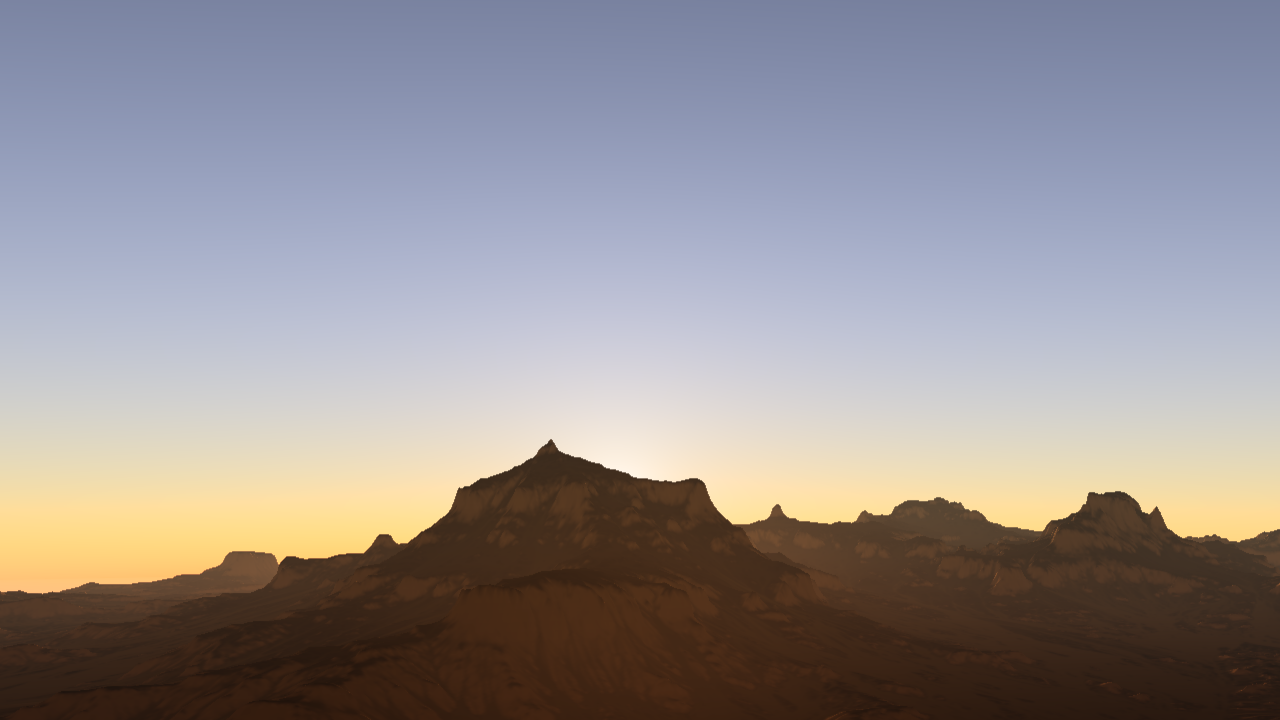
\includegraphics[width=\textwidth]{media/Sunset_with_ozone.png}
         \caption{Sunset with ozone absorption.}
         \label{fig:Sunset absorption}
     \end{subfigure}
     \quad
     \begin{subfigure}[b]{1.0\textwidth}
         \centering
         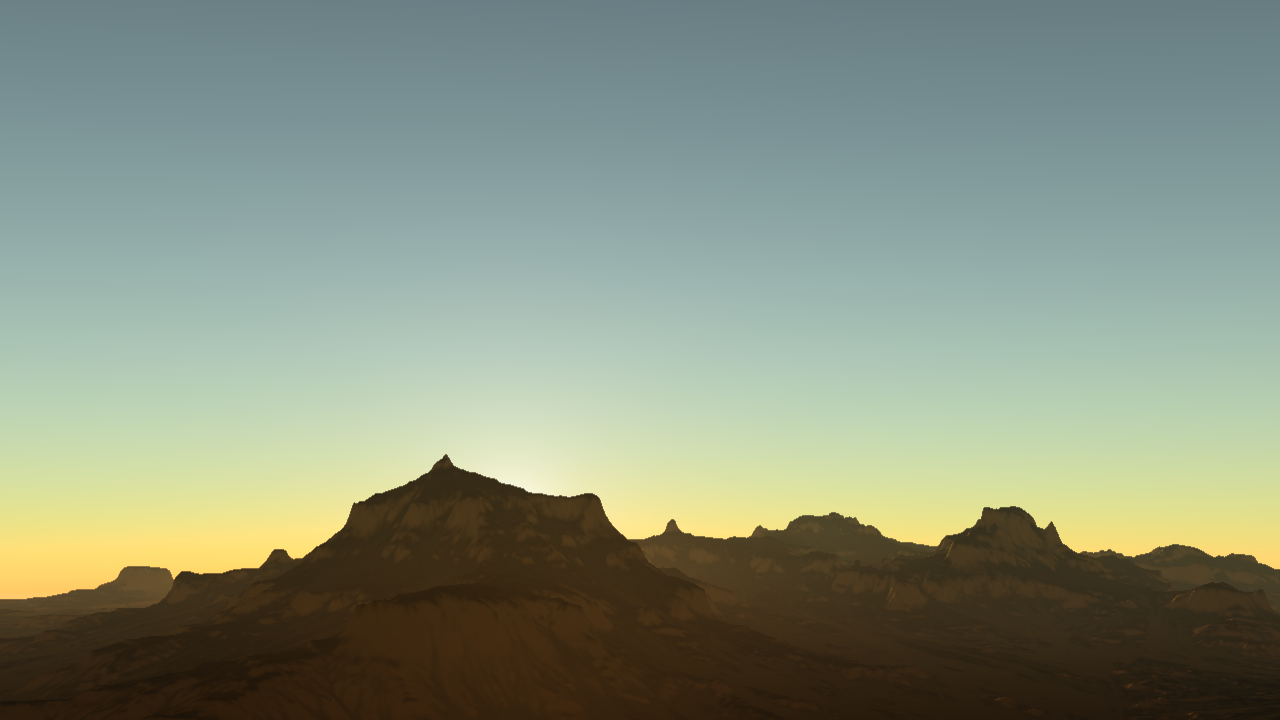
\includegraphics[width=\textwidth]{media/Sunset_without_ozone.png}
         \caption{Sunset without ozone absorption greenish tint can be visible.}
         \label{fig:Sunset no absorption}
     \end{subfigure}
        \caption[Ozone absorption effect]{Images showing the difference the absorption effect of ozone and oxygen makes on the atmosphere
        look during sunset.}
        \label{fig:ozone oxygen effect}
\end{figure}

\chapter{Proposed solution}
First we describe the high-level overview of everything that happens during one frame. Along with this, we also provide 
additional details regarding the Look up table setup and parameterization. After that, multiple chapters will follow,
describing every step from the start all the way to the final image in more detail.

The process of rendering a single frame can be divided into four parts. These four parts directly map to four command
buffers which are submitted to the GPU each frame. The first command buffer is responsible for the computation
of the four LUTs used to render the atmosphere. The second command buffer renders all the objects and terrain. Along with this
the atmosphere, it's effects and clouds are also rendered. After this, the third command buffer is executed. The main function of this 
command buffer is to map values from the HDR range into LDR that is used by the image presented to the screen.
Lastly, the fourth command buffer containing commands used to render the UI controlling various parameters of the atmosphere
and clouds.

We have one more command buffer responsible for the computation of the Worley noise texture described in 
Section~\ref{Worley noise LUT}. Since this computation can be expensive, we decided not to submit this
buffer each frame but instead only during the first frame.

\section{Atmosphere Precomputations}
As mentioned above, to speed up the time taken to render the atmosphere, it is beneficial
to precompute certain parts of the rendering equation and store them in multidimensional tables.
In this work, an LUT setup proposed by \cite{hillaire_2020} is used. The following section will provide a description of this model.

\subsection{Transmittance LUT}\label{transmittance computation}
First introduced by~\cite{bruneton_neyret_2008} this LUT is used to store the Transmittance $T$
described in Section~\ref{extinction over a finite path} (specifically Equation~\ref{eq:transmittance}).
When the atmosphere is ray-marched, the value of $T$ is used very frequently to model the atmosphere attenuating
the passing light. However, to compute this value, a second ray must be traced towards the light source, which
can be very expensive. Given the above conditions and the overall smooth distribution of atmospheric transmittance
it is beneficial to precompute Transmittance value for the entire atmosphere and store it into a table.

In this model, the spherical symmetry of the atmosphere is considered. This means that the density 
of the atmosphere (and thus the scattering and absorption parameters of the atmosphere) only
changes with height. Given this assumption, we store the precomputed values into a 2D lookup table.
This LUT is parameterized as follows:
\begin{itemize}
    \item $x$ axis - map $x$ to a value between [0,1] by considering the distance $d$ to the top
                     atmosphere boundary, compared to its minimum and maximum values 
                     $d_{\mathrm{min}}=r_{\mathrm{top}}-r$ and $d_{\mathrm{max}}=\rho+H$
                    \cite{bruneton_neyret_2008}
    \item $y$ axis - the height above the surface normalized by the total height of the atmosphere 
                     is used
\end{itemize}
\begin{figure}
    \centering
    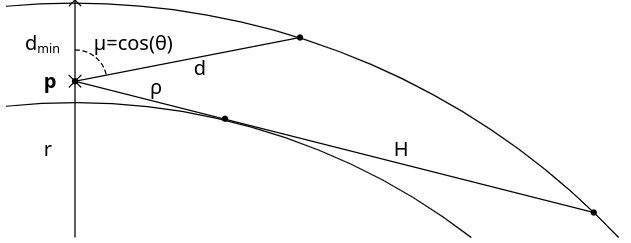
\includegraphics[width=0.7\textwidth]{media/transmittance_mapping.png}
    \caption[Transmittance LUT mapping]{Image taken from~\cite{bruneton_neyret_2008} showing the mapping of Transmittance LUT}
\end{figure}

Both parameters are in the range of [0,1]. Looking at the formula that specifies the parameterization of the coordinate x,
the range [0,1] can be easily deduced as we use the min and max values in the calculation. Similarly, the y 
parameterization range is apparent from the formula, as there is no point in storing values for heights
that are outside the atmosphere.

\subsection{Multiple Scattering LUT}
As described previously in Section~\ref{multiscatt approx}, in this work a new approach proposed by~\cite{hillaire_2020} is used.
The value of $\Psi$ (computed by Equation~\ref{transfer factor equation}), representing the contribution of isotropic multiplescattering to luminance, is stored in a 2D LUT. The parameterization is very similar to the
Transmittance LUT\@:
\begin{itemize}
    \item x = 0.5 + 0.5 cos($\theta$)
    \item y = $\frac{h - R_{Ground}}{R_{Top} - R{Ground}}$
\end{itemize}

\subsection{Sky-View LUT}\label{sky view LUT parametrization}
As noted by~\cite{hillaire_2020} the overall frequency of the image of the rendered atmosphere 
is very low. Because of this, it is possible to render the far sky into a latitude/longitude
texture that is of much lower resolution than the final image. It is possible to get good looking
results with Sky-View LUT sizes in orders of 10 times lower than the final resolution.

Because the highest visual frequency is introduced by the Sun (mostly) near the horizon, linear parameterization of this
LUT would produce artifacts in those high-frequency areas. To solve this Sky View LUT is
always oriented in a way such that the sun is present at the same position in the texture.
This then gives the option to map the values non-linearly by adding more samples to the areas of high 
change in frequency.

\begin{figure}
    \centering
    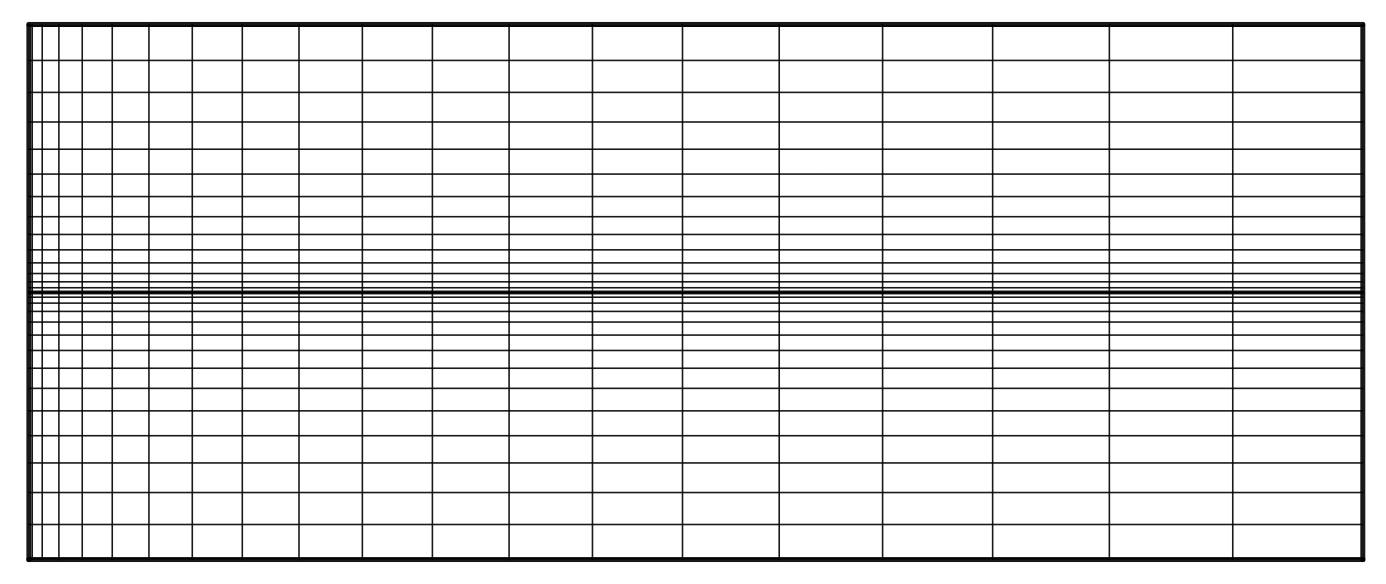
\includegraphics[width=0.9\textwidth]{media/sky_view_mapping.png}
    \caption[Sky View LUT mapping]{Visualization of the skyView mapping where sun moves up and down along the upper half of 
        y range but is always on the left border of the image and horizon is always a dividing line
        down the middle of the image}
    \label{fig:sky_view_mapping}
\end{figure}

\begin{itemize}
    \item $x$ axis - A quadratic curve is used (longitude $lon$) $x = \bigg(\frac{lon}{\pi}\bigg)^{2}$
                     giving more samples to the left side of the image where the sun is positioned
    \item $y$ axis - A quadratic curve is used (latitude $lat$) 
        $y = 0.5 + 0.5 \cdot sign(lat) \cdot \bigg({\frac{|lat|}{\pi / 2}}\bigg)^{2}$
\end{itemize}
where $lon$ is in the range [-$\pi$/2, $\pi$/2] and $lat$ is in the range [0,$\pi$]. Because we are 
modeling the planet with the assumption that it is perfectly spherical, the latitude range of
[0,~$\pi$] is identical to [0,~-$\pi$]. This is also the reason why in Figure~\ref{fig:sky_view_mapping}
only half of the Sun is mapped into the target texture.


\subsection{Aerial Perspective LUT}
\label{aerial perspective}

The Aerial perspective refers to how we see objects as they recede into the distance from the viewpoint.
This effect can be seen, for example, when looking at distant hills. As the distance of the hills from
the viewing position increases, the contrast between the hills ant their background is reduced along 
with the contrast of any landmarks.

To simulate this effect, a 3D lookup table is precomputed. To parameterize along the z-axis, we use the 
distance from the viewing position. At each depth level, a 2D LUT is fitted to the camera view frustum.
Each layer of the Aerial Perspective LUT contains the atmosphere luminance and average transmittance at the corresponding depth. The 
computation of each layer is almost identical to the Sky View LUT. The only difference being that we do not ray march all
the way to the edge of the atmosphere but stop at the depth of the corresponding slice.
This LUT is then applied as the last step in the sky and cloud rendering process.


\section{Cloud Precomputations}
\label{Worley noise LUT}

\begin{figure}[h]
    \centering
    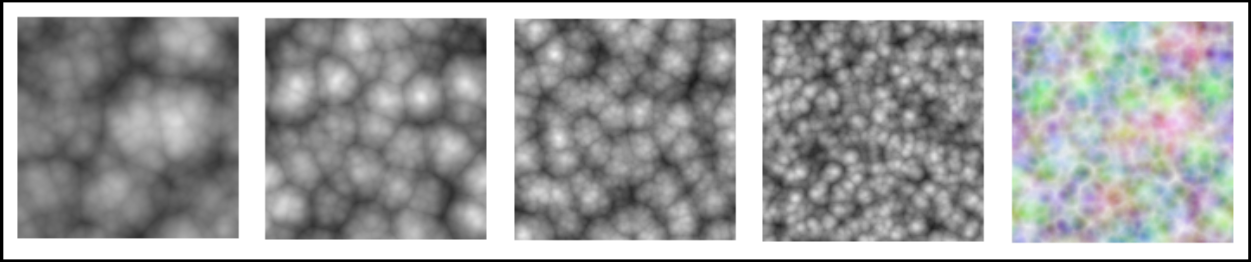
\includegraphics[width=1.0\textwidth]{media/worley_noise_high_res_showcase.png}
    \caption[Worley noise showcase]{From left to right separate RGBA channels storing worley noise and all of the
    channels combined together in the right most image}
\end{figure}

As already stated, the very popular method of rendering clouds by~\cite{schneider2015real}, which this work also uses,
relies on the usage of inverted Worley noise. Computation of non-inverted Worley noise can be split into two parts.
First, a number of points is randomly distributed in a desired area resp.~volume for 2D resp. 3D texture. 
After this, for each texel resp.~voxel in the desired area, the distance to the
nearest point was calculated and stored. Inverting Worley noise simply consists of storing 
$max\_distance - distance$ where $max\_distance$ is the maximum possible distance between a point
and a texel, respectively. voxel and $distance$ is the distance from currently processed texel resp.~voxel towards
the nearest point. 

One possible approach could be to scatter those points at random throughout the atmosphere
and then compute the nearest distance during the raymarch of the cloud. Although this approach 
would work, it would be very slow to compute. To decrease the computation time, 
a technique proposed by~\cite{schneider2015real} uses multiple 3D textures that have
precomputed Worley noise with various frequencies stored in them. Those textures are then sampled
during the raymarch of the cloud, providing a significant increase in speed.

The method implemented in this work is based on the implementation described by~\cite{lague_2019}. It uses two 4-channel
16bit float textures. Both textures store separate Worley noises with increasing frequencies in each of the 
RGBA channels. The red channel then stores Worley noise with the lowest frequency and the alpha
channel stores noise with the highest frequency.

The texture will have to be tiled multiple times to cover the entire skydome. This gives another
requirement for the texture to be tileable (seamless) along all three dimensions. 

\chapter{Implementation}
This chapter describes how the LUTs described in previous chapters are computed and used to produce the final image.
As in most performance-dependent applications, this work was implemented using C++. Vulkan API was used as an 
interface with the GPU. Multiple factors played a role in deciding on the graphics API that would
be used. One of the goals of this work was to provide a multiplatform solution 
(targeting Linux and Windows), which ruled out the use of DirectX almost immediately leaving only
OpenGL and Vulkan. While OpenGL is more friendly in terms of the API, it was decided to instead use
Vulkan and pay the price of more upfront work (and LOC) in setting all of the things handled by OpenGL's
driver side and in return get the performance benefits of more manual control over GPU exposed by Vulkan.

\section{Application resources}
In this section, we describe all the application resources and their format. We will mostly omit small uniform 
and storage buffers used only for parameterization, as they are multiple orders smaller than the LUT textures and have 
no real effect on the memory requirements of the application. Please note that, if not mentioned otherwise, each 
resource is allocated once for each \textit{frame in flight} we want to have.

\subsection{Atmosphere and clouds}
When rendering the atmosphere four previously described LUTs have to be computed. We use 16 bit RGBA texture
for each LUT. The parameterization that we decided to use can be seen in Table~\ref{tab:Atmosphere LUT}. 
\begin{center}
\begin{table}[H]
\begin{tabular}{ ||c|c|c|| } 
\hline
Look up table & Resolution & size in bytes \\
\hline
Transmittance LUT & 256 $\times$ 64 & 128 KiB \\
\hline
Multiscattering LUT & 32 $\times$ 32 & 8 KiB \\
\hline 
Sky View LUT & 192 $\times$ 128 & 198 KiB \\
\hline
Aerial Perspective LUT & 32 $\times$ 32 $\times$ 32 & 256 KiB \\
\hline
Total & & 590 KiB \\
\hline
\end{tabular}
\caption[Atmosphere LUT sizes]{\label{tab:Atmosphere LUT} Parameterization and sizes of LUT's used to render atmosphere.}
\end{table}
\end{center}

In addition to this we use two volumetric textures used to store Worley noise. Similarly to LUT's used to render atmosphere,
these textures store 16 bit floating point values in each of the channels. The parameterization along with the size can be seen 
in Table~\ref{tab:Noise LUT}. The resolution of the noise textures is slightly higher than described by~\cite{schneider2015real}.
We felt like it gave us higher quality results with less visible tiling, but it could easily be lowered to half or more and
still produce good looking results. 
\begin{center}
\begin{table}[h]
\begin{tabular}{ ||c|c|c|| } 
\hline
Look up table & Resolution & size in bytes \\
\hline
Base Shape Noise LUT & 256 $\times$ 256 $\times$ 256 & 128 MiB \\
\hline
Detail Noise LUT & 128 $\times$ 128 $\times$ 128 & 16 MiB \\
\hline 
Total & & 144 MiB \\
\hline
\end{tabular}
\caption[Clouds Noise LUT sizes]{\label{tab:Noise LUT} Parametrization and sizes of LUT's used to store Worley noise.}
\end{table}
\end{center}

\subsection{Sky}
Because our implementation uses HDR as it's preferred format, we need a texture capable of
storing HDR values throughout the process of rendering a frame. For this purpose we use
one 32bit floating-point RGBA texture with the same resolution as swap chain images.
We also make use of two depth buffers during each pass. Because we make no use of stencil buffer,
we decided to use one channel 32bit depth format for each depth texture. The memory requirements
for both 720p and 1080p resolution can be seen in Table

\begin{center}
\begin{table}[H]
\begin{tabular}{ ||c|c|c|| } 
\hline
Texture & Resolution & size in bytes \\
\hline
720p HDR Backbuffer & 1280 $\times$ 720 & 14.1 MiB \\
\hline
720 Depth buffers & 1280 $\times$ 720 $\times$ 2 & 7.05 MiB \\
\hline 
Total & & 21.15 MiB \\
\hline
\hline
1080p HDR Backbuffer & 1920 $\times$ 1080 & 31.65 MiB \\
\hline
1080 Depth buffers & 1920 $\times$ 1080 $\times$ 2 & 15.82 MiB \\
\hline 
Total & & 47.5 MiB \\
\hline
\end{tabular}
\caption[HDR backbuffer sizes]{\label{tab:Backbuffers} Parameterization and sizes of HDR backbuffers}
\end{table}
\end{center}

\section{Main Draw Loop}
\label{Main draw loop}
Because most of the command buffers in our implementation are pre-recorded and do not need
rebuilding, the main purpose of the draw loop is to keep the GPU fed with as much work as possible. 
In order to do this, Vulkan allows us to submit work for multiple frames in advance, which means that
we can render a new frame while the previous frame is still in the process of rendering.
We will refer to this concept as having multiple \textit{frames in flight}. By default, three frames
are in flight in our implementation (which is incidentally also the amount of swap chain images we create).

There are multiple caveats to having multiple frames in flight. First, we have to ensure
that the work submitted to the GPU is actually finished in time. If we do not do this and the GPU
is slower in executing the command buffers than the CPU is in submitting them, the corresponding
command queues will fill slowly and eventually overflow. Another thing we need to avoid is two (or more)
frames in flight that are modifying this resource in any way. 
modified during the rendering process. To avoid this, multiple GPU-GPU and CPU-GPU synchronization
points are implemented in a similar fashion as described in~\cite{overvoorde_2021}.

At the start of our loop, we check if we do not already have more images in flight than we
want. For this purpose, we create a fence for each frame in flight that we want to have. When we are
sure that the number of frames in flight is less than the maximum specified values, we continue by
acquiring the next image index from the swap chain. This prevents the above-mentioned issue of 
slowly overflowing our command queues.

\begin{figure}
    \centering
    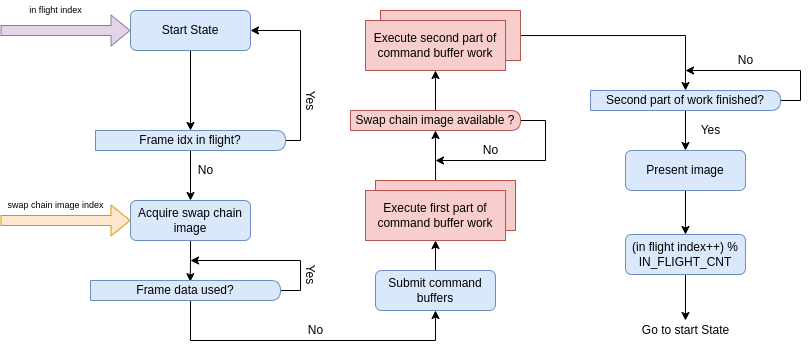
\includegraphics[width=1.0\textwidth]{media/Thesis_main_draw_loop.png}
    \caption[Main loop flow diagram]{Flow diagram of the draw loop execution order. CPU parts as well as CPU-GPU synchronization
    points are colored blue. Similarly GPU parts and GPU-GPU synchronization are colored red}
    \label{fig:main loop exec diag}
\end{figure}

If we specified more maximum frames in flight than there are swap-chain images or if the swap-chain
returned image indexes out of order, the previous fence would not stop us from 
ordering the GPU from using the same set of data for multiple frames. Because of this, we have an
array of structures containing all of the data that change during the process of
rendering one frame and a fence specifying whether the data are currently being used by some
in flight frame. Whenever a new image is acquired from the swap chain it checks the 
corresponding frame data structure fence and only after the fence has been signaled an appropriate
command buffer is submitted to GPU. Whenever we finish rendering of any frame, a structure 
fence is signaled, allowing another frame to be submitted. Figure~\ref{fig:main loop exec diag} shows
a flow diagram visualizing the entire draw loop.

For each frame, four command buffers are submitted to the GPU. The first pair of command buffers can start executing immediately, 
but since the second pair of command buffers writes directly into a swap chain image, we need to make sure the
corresponding image is available for us to write. We use an additional array of semaphores. Each semaphore is signaled
when the presentation engine is finished using the corresponding image.


\section{Command buffer descriptions}
In this section, we will provide a fairly detailed description of the commands that are submitted 
in each command buffer. We will also describe the GPU-GPU synchronization that takes place inside
each of the command buffers. Think of this section as a description of Vulkan specific
parts in our implementation. This, of course, is not everything that is Vulkan specific in our
application; however, as we did not believe those other parts unique to our implementation, we 
decided to omit them.

\subsection{LUTs command buffer}
\begin{figure}
    \centering
    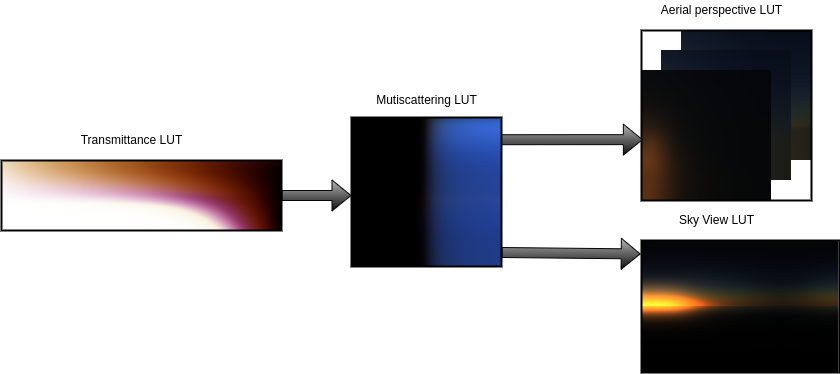
\includegraphics[width=0.9\textwidth]{media/LUT_execution_order.png}
    \caption[Sky LUT draw order]{The order in which individual Sky Luts are drawn. Please note that color values of
    LUTs have been scaled in order to be properly visible}
    \label{fig:LUTs execution order}
\end{figure}

When pre-computing LUT entries most of the graphics pipeline's features
would get in our way instead of helping us. Due to this in our implementation, we
decided to use compute shaders to fill out all LUTs. Each LUT is computed by one
shader in one dispatch. 

\begin{figure}
    \centering
    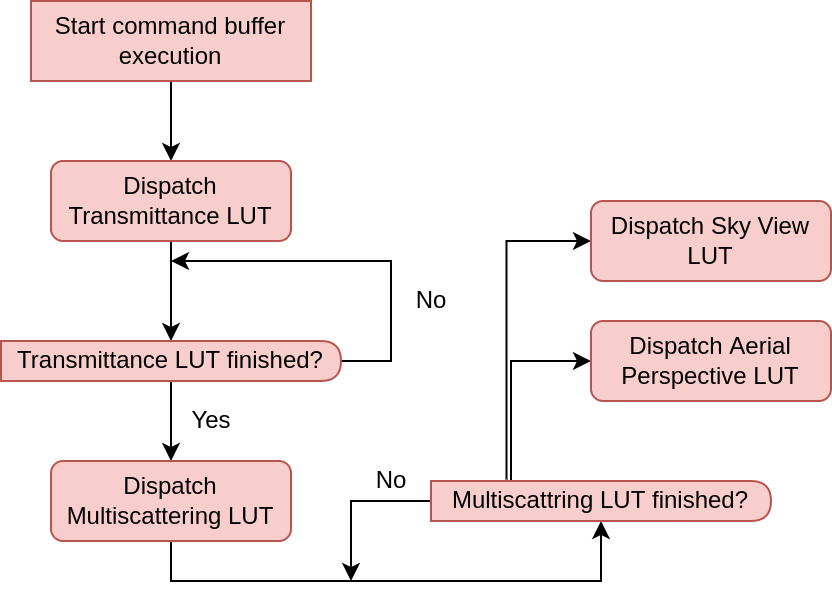
\includegraphics[width=0.9\textwidth]{media/LUTs_command_buffer.png}
    \caption[LUT command buffer dependencies]{Flow diagram showing dependencies between individual operations in LUTs command buffer.
        As all parts are either executed on GPU or are GPU-GPU synchronization they are all marked red}
    \label{fig:LUTs command buffer}
\end{figure}

Compute dispatch commands are recorded in the order shown in Figure~\ref{fig:LUTs execution order}
in the command buffer. Because the intermediate results of Transmittance LUT are needed when filling
Multiscattering LUT and similarly intermediate results of Multiscattering LUT are needed when calculating
SkyView and Aerial perspective LUTs we need to introduce some sort of synchronization between the
individual dispatch commands. We decided to use pipeline barriers for this. This results in us waiting,
after each drawcall, utill all of the previously submitted compute work has been finished before
issuing another dispatch. Figure~\ref{fig:LUTs command buffer} shows the visualization of
the execution order in this command buffer, as well as the synchronization performed between executions.

\subsection{Worley Noise command buffer}
As described in Section~\ref{Main draw loop} sometimes an additional LUT command buffer may be submitted.
This command is used to compute the 3D Worley noise texture used in later phases. Similarly to the 
previous section we have no use for graphics pipeline's features when generating this texture, so we
use compute shaders here as well.

We decided to follow the approach used by~\cite{lague_2019} and render the texture in two separate passes.
The first pass renders the Worley noise itself, and the second pass normalizes the values to the range between 
0 and 1. Since each channel of the resulting 3D texture stores completely separate Worley noise, we decided
to use a separate one-channel texture for each of the final four textures in the first pass. We use 
these four textures as input to the second pass, which normalizes and combines them by storing values
from each texture in the corresponding channel.

As far as we know, it is not possible to write only one channel of a texture at a time from compute shaders.
For this reason if we only used a single texture each dispatch would have to read the value previously stored
in all of it's channels, modify single channel, and write back values for all four of these channels. In addition
to loading unused data from VRAM we would also have to introduce synchronization between dispatches writing into
separate channels to avoid write after write hazards etc\dots 

\begin{figure}
    \centering
    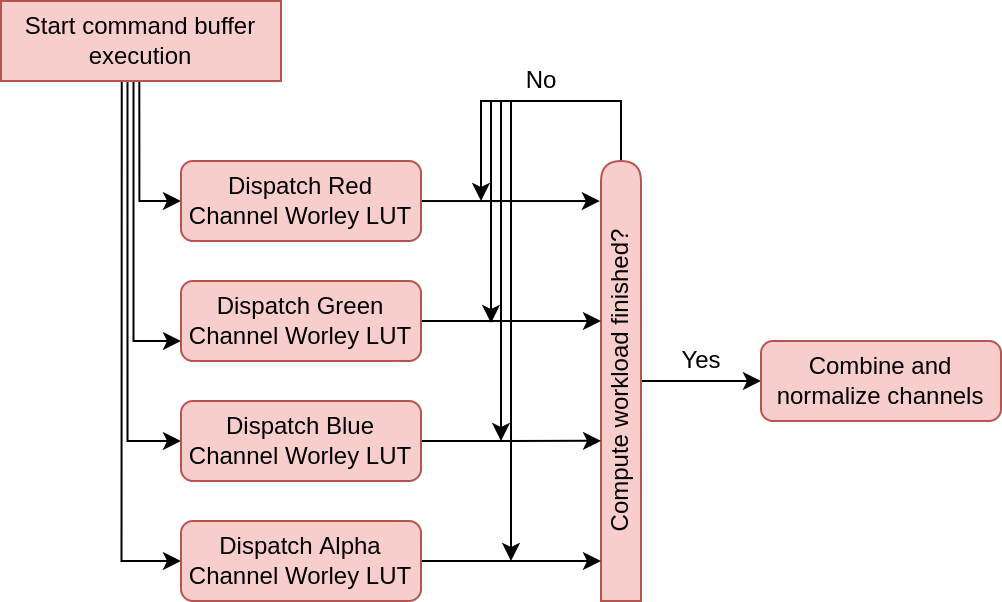
\includegraphics[width=0.9\textwidth]{media/Worley_command_buffer.png}
    \caption[Worley command buffer dependencies]{Flow diagram showing dependencies between and execution order of worley noise command buffer}
    \label{fig:worley command buffer}
\end{figure}
By splitting the texture into four separate textures in the first pass, we avoid all of the problems described above.
We don't need any kind of synchronization between the writes to a separate texture. Only synchronization that
we must ensure happens is the one between the first and second pass. To ensure this, a single pipeline barrier
is inserted making sure all writes and reads in compute shader stage by previously called dispatches have finished
before we normalize and combine all channels together. The entire execution process can be seen in
Figure~\ref{fig:worley command buffer}

\subsection{Sky command buffer}
\label{Sky command buffer}
When all LUTs have been precomputed, we can move on to rendering all the objects we want
in our scene and drawing the sky (atmosphere) with clouds. The ordering here is important; we
first need to render all the objects before drawing the sky and clouds. This is because drawing 
sky, clouds, and atmosphere requires depth information about the rest of the scene.

As mentioned above after all scene objects were rendered far sky is drawn to the sections
of the image which have maximum depth value still stored, meaning no object is occluding the view.
After this, the clouds are rendered.
Whenever scene object is only partially occluded by cloud (as an example we can imagine tops of mountains poking into
the bottom of the cloud layer), we don't want the object to fully disappear. In order to properly
display this effect, we will require a scene depth buffer as well. Lastly, the aerial perspective is applied.
Recall that in Section~\ref{aerial perspective} we define the aerial perspective as a reference
to how we see objects as they recede into the distance. With this definition in mind, it is now clear why we need scene
depth information during this rendering phase as well.

\begin{figure}
    \centering
    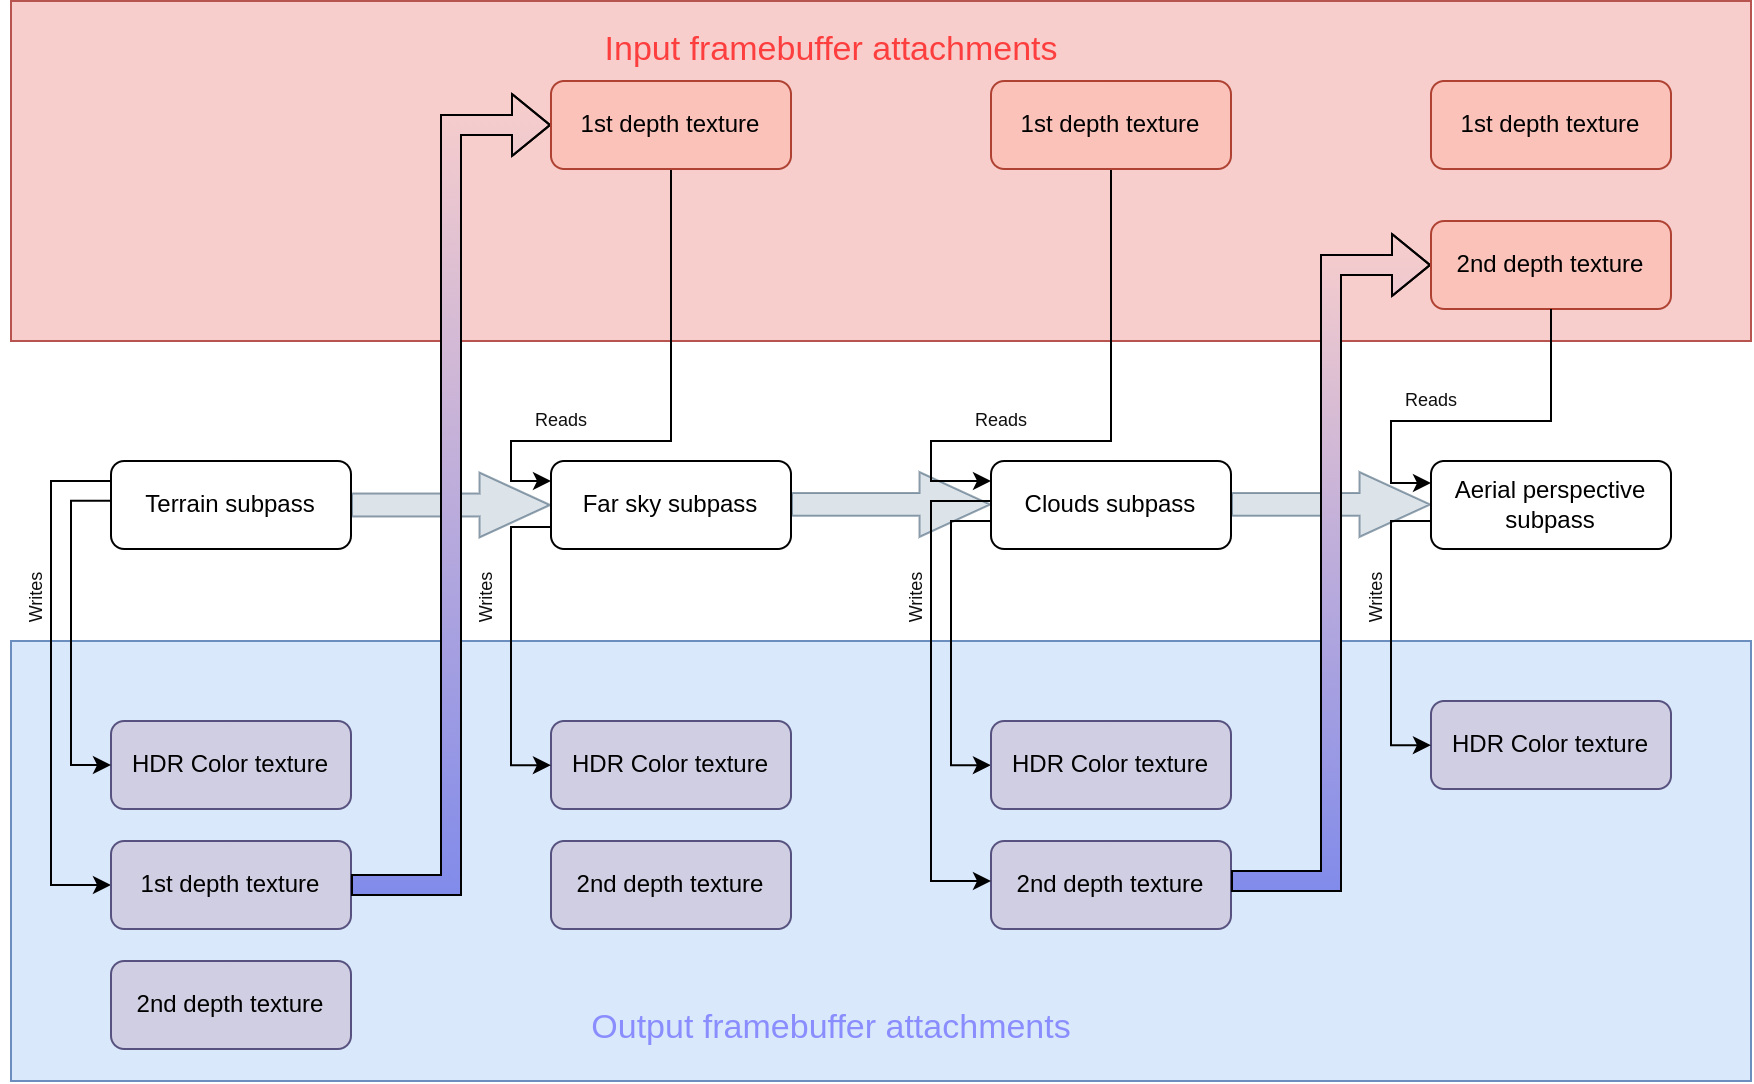
\includegraphics[width=1.0\textwidth]{media/Sky_render_read_write_dependencies.png}
    \caption[Supass reads and writes]{Visualization of writes and reads performed by each subpass. Additionally we also show
    when do transitions from output attachment into input attachment inside a framebuffer occur }
    \label{fig:Sky render read write deps}
\end{figure}

There is one problem. We would like to apply aerial perspective coherently to the entire scene. Clouds, however,
are part of the scene, so we want to draw the effects of aerial perspective on top of the clouds as well.
To do this, we need information about how far the clouds are from the viewing point stored
in the depth texture. But above we mentioned that clouds need depth texture as input as well. This would
mean that the pass rendering clouds wants to read and write the same texture. To avoid this problem,
we introduce a second depth texture. When rendering clouds, we then read from the first texture which contains depth
values of scene objects combine with depth values of the clouds and write the result into the second texture.
The second texture is then used as input into the aerial perspective pass. Figure~\ref{fig:Sky render read write deps}
shows how every subpass reads or writes resources from the framebuffer.

\begin{figure}
    \centering
    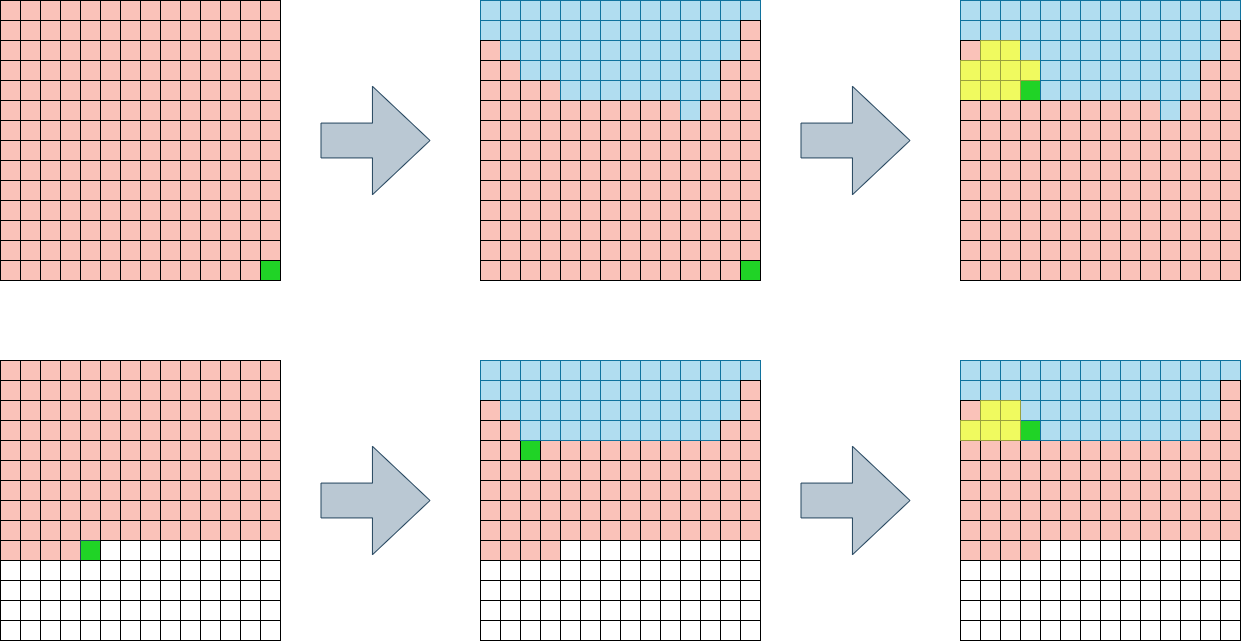
\includegraphics[width=1.0\textwidth]{media/Local_vs_global_dependencies.png}
    \caption[Local vs global dependencies]{The top sequence shows traditional style of rendering, where we wait to render
    the entire image before continuing with next pass. Fragment highlighted in green shows 
    which position current dispatch is shading. We can see that only third pass is active 
    and previous passes already finished (visualized by active fragment being in the low right corner). 
    Bottom sequence shows how local dependencies could render image. We can see that all three passes
    are rendering at the same time but only on the fragments which were already processes by previous
    passes}
    \label{fig:local vs global dependecies}
\end{figure}

Similarly to LUT computation, we need to introduce GPU-GPU synchronization between individual
draw calls to make sure the previous part of the rendering has finished. However, we can be less strict
in this case. Because we know that in each pass of the sky rendering process we will be accessing the 
same \textit{framebuffer fragment region} (think fragment), we do not need to wait for the previous pass to finish 
the entire draw workload. We can instead just make sure that the previous pass has completed all the 
writes or reads of the \textit{framebuffer fragment region} we are currently processing. This gives
us the option to, for example, start drawing clouds before the entire far sky has been rendered.
We only instruct the GPU to make sure that all operations performed by previous passes above the current
\textit{framebuffer fragment region} are finished before the current pass reads or writes any values.

Note that we cannot make the same assumption when computing LUTs. There are multiple reasons for this, 
but the main ones are as follows:
\begin{itemize}
    \item 1. We have no way of knowing which LUT regions will be accessed by the following stage
    \item 2. We use different texture types (2D and 3D) as well as sizes for each LUT so we 
             are unable effectively unify them into a single framebuffer.
\end{itemize}

Because the entire sky-draw process reads and writes the same three textures, we do not need to specify a
separate framebuffer for each pass. The only thing that changes between the passes is how the framebuffer
textures are used. Luckily for us, this specific case is common enough that Vulkan exposes certain parts
of it's API just for this purpose, which are called subpasses and subpass local dependencies.

\begin{figure}
    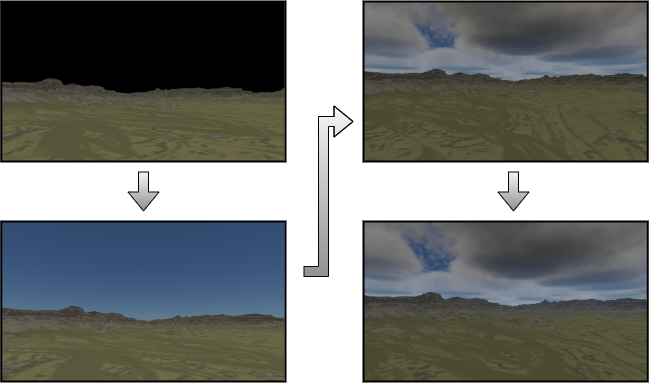
\includegraphics[width=1.0\textwidth]{media/Supass_process.png}
    \caption[Subpass stage changes visualization]{ This image shows how the image changes in each of subpass stages.}
    \label{fig:subpass process}
\end{figure}

A subpass represents single phase of rendering that reads and writes a subset of the attachments in a
render pass as well as describing the layout transitions and dependencies between multiple subpasses.
A subpass dependency is essentially an automatically inserted pipeline barrier at the start or 
end of each subpass. A subpass local dependency (or dependency by region) is a type of 
subpass dependency that is only framebuffer local. A framebuffer-local dependency is exactly what
we described above, where separate subpasses only access the same \textit{framebuffer fragment region}.

We use a single render pass to render the sky. This render pass is divided into four sub-passes. Each subpass is responsible for
one of the previously described phases in the described order:
\begin{enumerate}
    \item subpass - draw all scene objects
    \item subpass - draw far sky
    \item subpass - draw clouds
    \item subpass - draw aerial perspective effects
\end{enumerate}

Local dependencies between each subpass are specified as follows. First, since every subpass writes into the same HDR 
framebuffer attachment, we need to make sure to avoid write after write hazard. This can be solved
by inserting a local dependency guarding writes to a color attachment.

In addition, far sky and cloud supbasses read from the first depth attachment written by scene 
objects subpass. Similarly, aerial perspective subpass reads from the second depth attachment written
by clouds subpass. To prevent a read after write hazard, additional subpass dependencies
are added, which make the start of fragment shader in a subpass wait before early and late fragment
tests (this is where all writes into a depth buffer occur) were finished by the previous subpasses.
In addition, specified subpass dependencies also take care of the attachment transitions from input
attachments to output, etc.\dots where needed.

\subsection{Post process and GUI command buffers}
Final two buffers submitted by the application each frame are buffers that contain the post-processing 
of the final image and the drawing of the UI. Post processing the image consists of tonemapping luminance 
values stored in HDR buffer into LDR range and gamma correction. For the purposes of tonemapping,
we first need to calculate the average luminance of the current image. We use a two-pass compute approach 
described by~\cite{tardif_2019}. 

In the first pass, a histogram of the luminance values in the image is constructed. The second pass reads
this histogram and calculates the weighed sum. This sum is then used to calculate the adaptive average
luminance of the scene. Our post process fragment shader then reads this average value and uses it 
for tonemapping.

The synchronization used in this command buffer is very similar to the one used during the LUT computation.
A pipeline barrier is inserted between constructing the histogram and calculating the 
average luminance, making sure that all compute stage writes have finished before reading anything.
A second pipeline barrier is inserted before tonemapping draw call to make sure the previous 
dispatch is done writing the average luminance. 

The last command buffer we will describe is the one that shows all the UI on the screen. It does not need
any kind of synchronization done by us, as everything is handled internally by the ImGUI 
implementation.

%=================================== SHADERS ==================================
\section{Shaders}

In this section, we describe how we implemented most of the shaders used in our application. Although
we tried to provide a pretty detailed description, we still had to omit some less important or
interesting parts. The complete code for all shaders can be found 
\href{https://github.com/MatejSakmary/RenderingAtmospheres/tree/main/ProductionReadyAtmospheresVulkan/shaders}{here} or in the attachment.
Shaders are written in GLSL. They are compiled along with the application into SPIR-V 
intermediate format and are loaded as a part of the initialization sequence of the application.

\subsection{Raymarch implementation}

\begin{figure}
        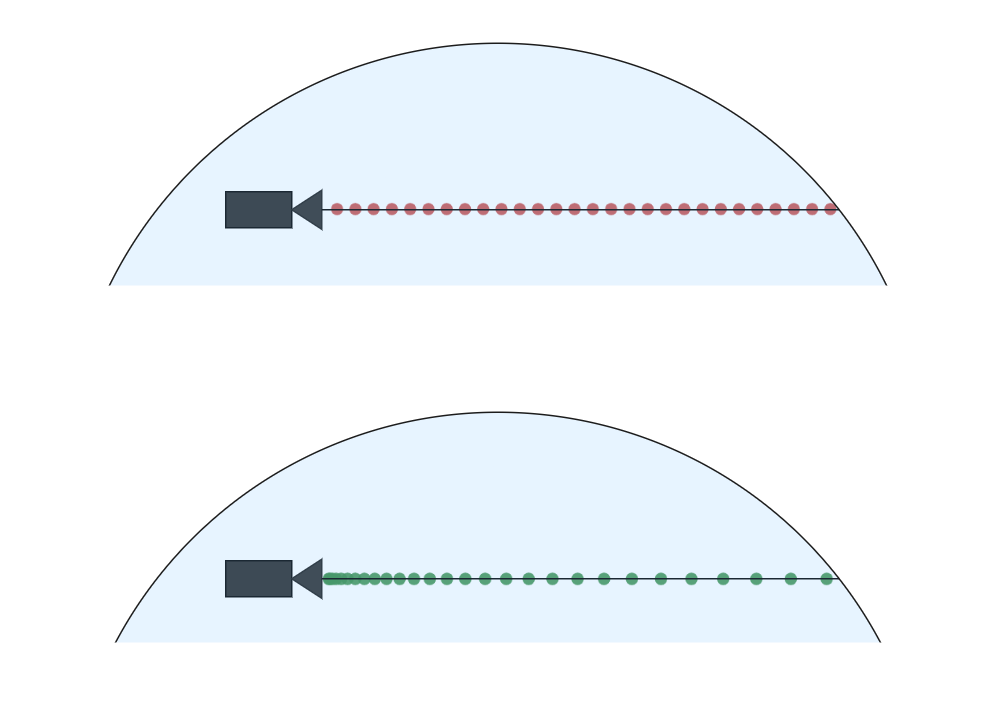
\includegraphics[width=0.7\textwidth]{media/Linear_vs_nonlinear_sampling.png}
        \caption[linear vs non-linear sampling]{In the top part of the image we can see linear sampling with constant distribution.
            Bottom part shows non-linear sampling with reducing sample density based on the
            distance from the ray origin}
        \label{fig:linear nonlinear samples}
\end{figure}

Ray marching is a key technique that many of our shaders use. Due to the frequency of it's appearance
in our implementation, we decided to dedicate a separate section to explain it. This makes it so that we can later
just refer to this subsection instead of duplicating it throughout the rest of the shader implementation section.
Whenever we use the function call \verb|raymarch(...)| or \verb|raymarch_nonuniform(...)| we refer to this section.

As hinted at in the previous paragraph, we make use of two different ray march functions. The difference
between those functions is the distribution of ray march samples along the ray. The first function
samples the path linearly, always moving by a constant offset. The second nonuniform function, as the name suggests, 
distributes the samples nonuniformally with a higher density of samples near the ray
origin. The further we go from the origin of the ray, the bigger steps we take along the ray. This can,
in some situations, lead to better looking images and generally nicer results.

\begin{lstlisting} [
    caption=Linear raymarch function,
    language=GLSL,
    label={lst:linear raymarch listing}
] 
// position of last step is stored here
vec3 oldPos = vec3(0.0, 0.0, 0.0);
vec4 raymarch(vec3 dir, vec3 pos, float iter, 
    float iterCnt, float rayLength)
{
    // Sample at one third of interval - gives better
    // results when integrating exponentional functions
    float rayShift = rayLength * (iter + 0.3) / iterCnt;

    vec3 newPos = pos + rayShift * dir;
    float dt = newPos - oldPos;
    oldPos = newPos;
}
\end{lstlisting}

In Listing~\ref{lst:linear raymarch listing} we can see our implementation of the linear ray march
function. Parameters \verb|dir| and \verb|pos| denote the starting position and direction of the 
ray. Following this \verb|iter| and \verb|iterCnt| are the current step index and the amount of steps
our ray will be divided into. Lastly, \verb|rayLength| is the distance over which we want to 
distribute our samples. 

\begin{lstlisting}[
    caption = Nonlinear ray march function,
    language=GLSL,
    label={lst:nonlinear raymarch listing}
]
vec4 raymarch_nonuniform(vec3 dir, vec3 pos, float iter, 
    float iterCnt, float rayLength)
{
    step0 = pow(iter / iterCnt, 2);
    step1 = pow(iter + 1.0 / iterCnt, 2);

    realStep0 = step0 * raymarchLength;
    // Make sure not to overshoot the raymarching distance 
    // in the last sample
    realStep1 = max(step1 * rayLength, rayLength);
    float rayShift = realStep0 + (realStep1 + realStep) * 0.3;

    vec3 newPos = pos + rayShift * dir;
    float dt = realStep1 - realStep0;

    return vec4(newPos, dt);
}
\end{lstlisting}

In Listing~\ref{lst:nonlinear raymarch listing} we can see the extra step 
of squaring the step size first, condensing more samples towards the origin position.

\subsection{Atmosphere and Sky LUT computation}
Unless stated otherwise, all shaders described in this section are largely based on the open source
code provided by~\cite{hillaire_2020}. However, it is important to note that the shaders provided
by Hillaire were written in HLSL. This meant that before using any shader, we had to port
it to GLSL first. An additional effort was made to refactor most of the code and provide slightly more
comments. 

\subsubsection{Transmittance}
Our transmittance LUT implementation is based on a freely available source provided 
by~\cite{bruneton_neyret_2008}. For each LUT entry, we ray march a single ray from a 
specified direction towards the end of the atmosphere. We use the linear \verb|raymarch()|
function for this purpose. During this, we sample the density of the atmosphere from 
which we calculate the extinction coefficient and transmittance exactly as described
in Section~\ref{transmittance computation}.

The only change we have made is that instead of ray marching three times separately for
\textit{rayleigh extinction}, \textit{mie extinction} and \textit{ozone extinction} we
ray march only once sampling all three values at the same time, thus reducing the 
computation time to almost one third.

\subsubsection{Multiscattering}
As described in previous chapters, multiscattering LUT samples rays uniformly distributed along a sphere.
We decided to follow the example provided by~\cite{hillaire_2020} and use a local team
of 64 threads for this purpose. Each local thread is assigned a ray direction based on its
index, and the ray marches (using \verb|raymarch(...)|) until it hits the ground or the end of the
atmosphere. During each step, we sample the scattering and extinction of the medium and
calculate $L_{2^{nd}order}$ and $f_{ms}$ as described in Equations~\ref{fms definition}
and~\ref{Lf definition}.

\paragraph{Sampling the sphere}
\begin{figure}
        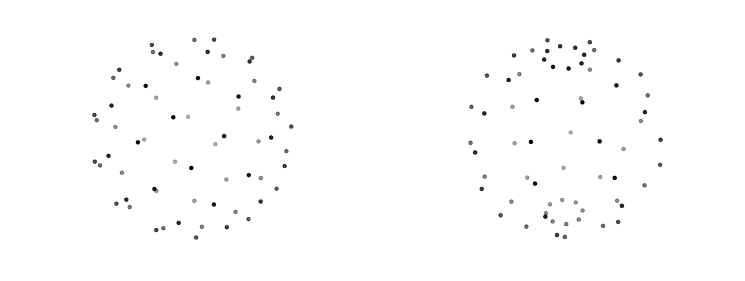
\includegraphics[width=1.0\textwidth]{media/Fibonacci_lattice_vs_Hillaire.png}
        \caption[Fibonacci lattice vs uniform sampling]{On the left distributing points using Fibonacci lattice. On the right
            distribution Hillaire uses in his implementation. Bias toward top and 
            bottom of the sphere is clearly visible}
        \label{fig:fibbonaci vs hill sphere}
\end{figure}

For distributing samples along a sphere, we used spherical coordinates. Previous solution
distributed samples using uniformly increasing angles $\theta$ and $\phi$. After this 
they were converted back to Cartesian coordinates by using a standard equation:
\begin{equation}
\label{eq:spherical to cartes}
    \begin{aligned}
        &x = \cos(\theta) * \sin(\phi) \\
        &y = \sin(\theta) * \sin(\phi) \\
        &z = \cos(\phi)
    \end{aligned}
\end{equation}
We decided to use a slightly better distribution along a sphere using \textit{Fibonacci lattice}
described by~\cite{gonzalez_2009}. Points are distributed along the sphere by the following 
equations:
\begin{equation}
    \begin{aligned}
        &\theta = \arccos\bigg( 1 - \frac{2n + 1}{N}\bigg) \\
        &\phi = \frac{2\pi n}{\Phi}
    \end{aligned}
\end{equation}

\begin{figure}
        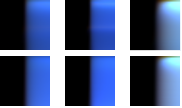
\includegraphics[width=1.0\textwidth]{media/sphere_sampling_multiscattering_comparison.png}
        \caption[Sampling effect methods]{The effects of sampling methods on Multiscattering LUT. Top row shows results when using
            Fibonacci lattice. Bottom row shows results of sampling used by Hillaire. From left to right
            Earth-like atmosphere, atmosphere with half of the particle density and atmosphere with 10x increased
            Rayleigh and Mie scattering coefficients. Colors were scaled for the results to be visible by 
            respective factors of 50, 20 and 100.}
        \label{fig:fibbonaci vs hill multiscattering}
\end{figure}
Where $\Phi$ is the golden ration defined as $\frac{1+ \sqrt{5}}{2}$. This produced samples that 
are less biased toward the top and bottom of the sphere, which can be seen in 
Figure~\ref{fig:fibbonaci vs hill sphere}. The effects of our sampling are compared to Hillaire's 
sampling in Figure~\ref{fig:fibbonaci vs hill multiscattering}. The differences are most visible
in the LUTs generated with a half-particle density. Reduced bias in sampling results in brighter values
when evaluating samples near the ground (top of the image). When using higher scattering coefficients,
the effect becomes very small, resulting in almost identical values.

\paragraph{Merging the results}
After every thread in the local workgroup finishes the ray marching loop, we need to merge the results
into a single value to be able to evaluate Equation~\ref{transfer factor equation}. In order
to do this, we create two local, group shared arrays the size of our work group (specifically 64 in our 
implementation). Each thread stores its $L_{2^{nd}order}$ and $f_{ms}$ values into those arrays 
using their local group ID as an index whenever it finishes ray marching.

Following this we use thread based merge to combine all of the results into two final values. We 
then use those values to calculate Equation~\ref{transfer factor equation} and store this result.
We can also see the code for this in Listing~\ref{lst:multiscattering merge}.

\begin{lstlisting}[ 
    caption=Multiscattering results merge,
    language=GLSL,
    escapechar=\%,
    label={lst:multiscattering merge}
]
                ...
// raymarch finished merging results (extra barrier
// is before this to ensure raymarch finish)
uint threadIdx = gl_localInvocationID.z;
if(threadIdx < 32)
{
    f_ms_shared[threadIdx] += f_ms_shared[threadIdx + 32];
    L_shared[threadIdx] += L_shared[threadIdx + 32];
}
// Make sure previous part of merge finished
groupMemoryBarrier();
barrier();
if(threadIdx < 16)
{
    f_ms_shared[threadIdx] += f_ms_shared[threadIdx + 16];
    L_shared[threadIdx] += L_shared[threadIdx + 16];
}

...

// we only want sigle thread past this point
if(threadIdx != 0) {return;}
//calculating Equation%~\ref{transfer factor equation}%
vec3 res = L_shared[0] * vec3(1.0 / 1.0 - f_ms_shared[0]);
imageStore(multiscatteringLUT, uv, vec4(res, 1.0));
\end{lstlisting}

\subsubsection{SkyView}
Calculating Sky View LUT is relatively simple. First, we transfer from uv
coordinates in the range [0, 1] to LUT parameters described in Subsection~\ref{sky view LUT parametrization}.
Because our ray march function uses Cartesian coordinates we first need to convert from spherical coordinates
(used by Sky View LUT parameterization). We use the same conversion as described in 
Equation~\ref{eq:spherical to cartes} giving us the direction of ray that we need to ray march. 

\begin{lstlisting}[ 
    caption=Multiscattering results merge,
    language=GLSL,
    escapechar=\%,
    label={lst:SkyViewLUT computation}
]
#define ITER_CNT 30;
void main()
{
    // Convert global invocation idx in range 
    // [0,skyViewRes] into uv range [0, 1] 
    vec2 uv = gl_GlobalInvocation.xy / skyViewLUTDim;

    // camera pos in UBO offset by groud radius 
    vec3 pos = getPos();
    vec3 dir = lutToDir(getLUTParams(uv));
    
    // get the ray intersection with the atmosphere
    float rayLen = getRayInt(pos,dir,atmoBounds);
    
    vec3 accumT = vec3(1.0);
    vec3 accumL = vec3(0.0);
    for(int i = 0; i < ITER_CNT; i++)
    {
        vec4 res = raymarch_nonuniform(dir, pos, i,
            ITER_CNT, rayLen);

        // res.xyz stores new pos, res.w stores step size
        float transIncRay = exp(-(medium.ext * res.w);
        vec3 light = calcLight(res.xyz, transIncRay); 

        accumL += accumT * light;
        accumT *= transIncRay;
    }
    // Store accumL into skyViewLUT 
    ...
}
\end{lstlisting}

Using this together with the current camera position in the world space, we ray march the full rendering
Equation~\ref{eq:complete rendering equation}. In order to produce better results, we use 
\verb|raymarch_nonuniform(...)|. Please note that we make use of the 
previously calculated Multiscattering LUT to evaluate orders of scattering higher than one.

A shortened version of the source code can be seen in Listing~\ref{lst:SkyViewLUT computation}.

\subsubsection{Aerial perspective}
\label{aerial perspective shader}
    Aerial Perspective LUT uses essentially the same computation as Sky View LUT, with few slight changes.
    First, because individual Aerial Perspective LUT layers are fitted on the view frustum in
    appropriate depth, we need to project from screen space coordinates into coordinates to get
    direction of the ray we want to ray march. The listing~\ref{lst:Screen to World} shows the code we
    use to achieve this. We first covert the screen coordinates into NDC coordinates. We the use
    the inverse of View-Projection matrix and divide by the new \textit{w} component to get 
    the position in the world space. To get the view direction, we take the vector from the camera to our newly
    acquired point and normalize it.

    We also limit the ray length to not be longer than the distance of the currently computed slice. 
    Using those slightly modified parameters, we execute the exact same ray march as used for the Sky View LUT
    computation. Lastly, we also store the average transmittance (averaged of all three wavelengths)
    in Alpha channel of each LUT layer. 

    \begin{lstlisting}[ 
        caption = Function transfer from screen coordinates into world direction,
        language=GLSL,
        escapechar=\%,
        label={lst:Screen to World}
    ]
    vec3 screenToWorldDir(vec2 uv, vec3 pos)
    {
        vec3 NDC = vec3(uv * vec2(2.0) - vec2(1.0), 0.5);
        vec4 Hpos = invViewProjMat * vec4(NDC, 1.0);
        vec3 dir = normalize(Hpos.xyz / Hpos.w - pos);

        return dir;
    }
    \end{lstlisting}
\subsection{Worley Noise computation}
Now we will describe the shaders used for both passes of our 3D inverted Worley noise generation adapted
from~\cite{lague_2019}. We use three octaves of noise with increasing frequencies, which are then
combined into a single noise using the standard Fractal Brownian Motion approach. During the generation
of each noise texture, we sample a unit cube filled with randomly scattered points. The naive approach 
of iterating through all points scattered in the medium to get the nearest point is very slow. 

To decrease the number of points that we need to check, we divide the unit cube uniformly into a set of smaller
cells, each containing a single point. By doing this, we guarantee that the nearest point will lie either in
the cell containing evaluated voxel or in one of its surrounding cells. For each voxel, we can then reduce the
number of checked points to only 28. To increase the frequency, we simply divide the unit volume into more cells. 

\begin{figure}
        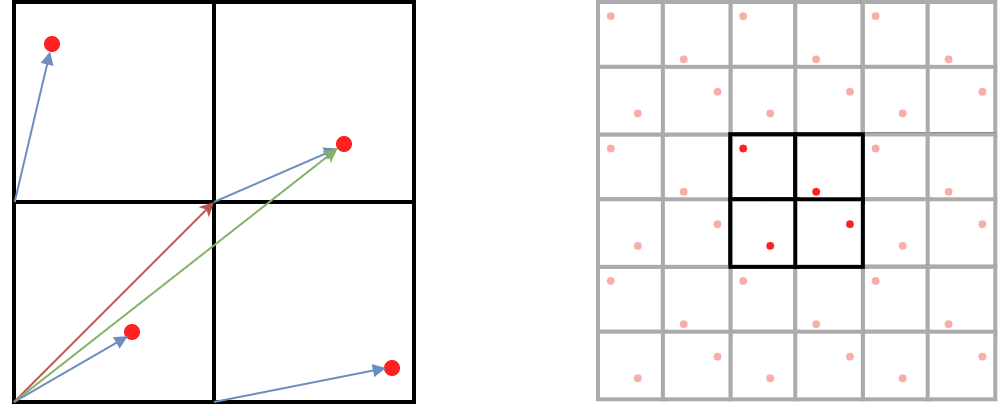
\includegraphics[width=0.7\textwidth]{media/Random_point_generation_worley.png}
        \caption[Worley offsets and mirroring]{On the left 2D unit volume with one division along each axis. Red arrow
            denotes cell offset, blue arrows denote cell local random offset and green
            denotes the global position of a point. On the right the same 2D mirrored volume 
            setup which produces seamless texture.}
        \label{fig:worley points distribution}
\end{figure}

To distribute the points randomly, we first generate an offset vector for each point in the local space of the cell.
This offset is then translated from the local cell space into the unit range global space by summing it with the
cell origin (front-bottom-left corner of the cell). Point generation is done on the CPU, after which we pass 
the point array to shaders as SSBO.

The increasing frequency is achieved by dividing the unit range into more cells. We generate three 
buffers of points, one for each octave of noise. To fulfill the seamless constraint, we must mirror the 
sampled volume and attach it to each side of our sampled volume. This, along with the local-to-global cell
mapping, can be seen in Figure~\ref{fig:worley points distribution}. The point data are actually not
duplicated; whenever we are near the edge, we just recalculate the neighbor index to the correct mirrored
cell.

\begin{lstlisting}[ 
    caption=Worley noise computation,
    language=GLSL,
    escapechar=\%,
    label={lst:Worley noise computation}
]
void main()
{
    vec3 index = vec3(gl_GlobalInvocationID.xyz);
    vec3 pixPos = index/texDimensions;
    // layer A, B and C corresponds to 1st, 2nd
    // and 3rd octave of noise
    float layerA = worley(0, pixPos);
    float layerB = worley(1, pixPos);
    float layerC = worley(2, pixPos);

    // combine all three octaves 
    float combinedNoise = layerA;
    combinedNoise += layerB * amplitude;
    combinedNoise += layerC * amplitude * amplitude;

    float localMax = 1 + amplitude +
         amplitude * amplitude; 
    // make sure the noise values are in the range [0,1]
    // and invert them
    combinedNoise /= localMax;
    combinedNoise = 1.0 - combinedNoise;
    atomicMin(minVal, combinedNoise);
    atomicMax(maxVal, combinedNoise);

    imageStore(...);
}
\end{lstlisting}

The code used to calculate one Worley noise texture can then be seen in Listing~\ref{lst:Worley noise computation}.
One thing we have not described yet is the pair of atomicMin and atomicMax on lines 22 and 23. Because
we are always sampling unit cube, the more divisions we have, the smaller the distances between individual points
will be. After inverting the values, this results in values that do not cover the entire range from zero to one.

As part of the second pass, we want to correct for this by remapping the values. However, in order for
us to do so, we need to know the max and min values which occur in the texture. This is exactly what the
code on lines 22-23 does, stores minimum and maximum values, which were written into the texture 
in another small SSBO.

\begin{figure}[h!]
        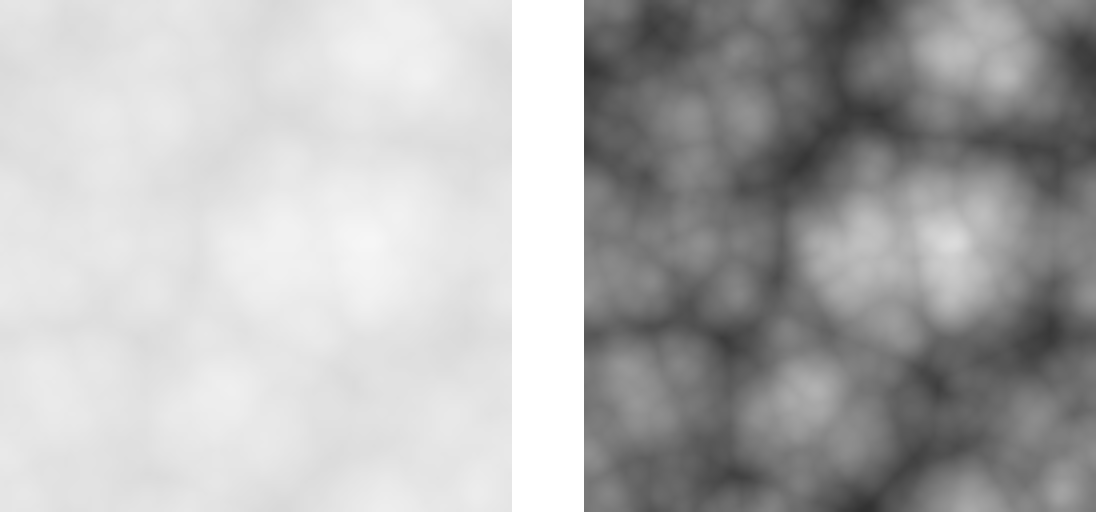
\includegraphics[width=0.7\textwidth]{media/Worley_raw_normalized.png}
        \caption[Worley normalization]{On the left raw values before normalization, on the right values after normalization.}
        \label{fig:worley normalization effects}
\end{figure}

The only thing that second pass then does is combine the four single-channel textures into a single
four-channel after normalizing the values. The code for this shader is presented in the 
Listing~\ref{lst:Worley noise normalization}, the effect of normalization of the noise can 
be seen in Figure

\begin{lstlisting}[ 
    caption=Worley noise normalization and combine pass,
    language=GLSL,
    escapechar=\%,
    label={lst:Worley noise normalization}
]
void main()
{
    float resultArr [CHANNEL_CNT];
    for(int i = 0; i < CHANNEL_CNT; i++)
    {
        float noise = loadVal(uv, i);
        float normNoise = (noise - minVal[i])/
                          (maxVal[i] - minVal[i]);
        resultArr[i] = normNoise;
    }
    vec4 result = vec4(resultArr[0],resultArr[1] ... ); 
    // Store the result in final texture
}
\end{lstlisting}

\subsection{Frame composition}
In this subsection, we will describe all shaders that are used to draw the HDR image that is used later
in post processing. We describe the shaders in the order of execution described in~\ref{Sky command buffer}.
Thus, each shader directly maps to a draw call executed in each subpass. Unless otherwise stated, the shaders described
in this section are again adapted from~\cite{hillaire_2020} and~\cite{lague_2019} and modified in some
places to fit our application.

\subsubsection{Terrain}
To draw the terrain, we first generate a subdivided unit length rectangle of points on the CPU. We use
these points as input to the vertex shader. For each vertex, we then sample the height map texture and offset 
the height by the sampled value. Lastly, we scale the model using the model matrix.

In the fragment shader stage, we use \textit{Phong reflection model}. Normals are read from a normal map
texture. To get the color of each fragment, a color mask map is used. Each channel of the color-mask map
corresponds to the weight of a single color. We multiply each of the four terrain colors by the sampled weight.
To get the color of the sun light hitting the terrain we sample Transmittance LUT giving us the colored 
transmittance towards the Sun. Please note that our Transmittance LUT only stores the transmittance
of the atmosphere and does \textit{not} include the transmittance of the cloud layer.

\subsubsection{Far sky}
The shader for drawing the far sky is also relatively simple. First, we check if the value stored in depth buffer
written by previous subpass is equal to the clear color. If it is, we know there are no objects obstructing 
the view and we can continue by drawing the sky. Otherwise, we do not draw anything and return early.

In order to sample the Far Sky LUT we need to convert the screen space coordinates into latitude and 
longitude used for Far Sky LUT parameterization. This step is exactly the same as the one used when
calculating the Aerial Perspective LUT. In fact, we can think of the Far Sky LUT as a last layer of Aerial
Perspective LUT with higher resolution, which is not fitted to the camera frustum but instead fitted
to the entire viewing range. Because of this similarity we will not describe the calculation used
to transform from screen space to world space and instead refer to 
Section~\ref{aerial perspective shader} where this process is explained.

To get Sky View LUT parameters, we need to know the angle of our ray from the horizon and the angle of 
our ray to the Sun. To get the angle to the Sun, we project both sun direction and view direction vectors onto
the xy plane and calculate their dot product. The angle from the horizon is given by the dot product
of the up vector with view direction vector. We can see this computation in Listing~\ref{lst:Screen to SkyView}. 
In the next step, we perform the inverse mapping of Sky View LUT to get the texture UV coordinates. As a last
step, we sample the Sky View LUT with our calculated UV coordinates and store the sampled value.

\begin{lstlisting}[ 
    caption=Screen position to Sky View LUT UV,
    language=GLSL,
    escapechar=\%,
    label={lst:Screen to SkyView}
]
vec2 posDirToLUTParams(vec3 pos, vec3 dir)
{
    vec3 up = normalize(pos);
    float horizonAngle = acos(dot(dir, up));

    vec3 dirProj = normalize(vec3(pos.xy, 0.0));
    vec3 sunProj = normalize(vec3(sun_dir.xy, 0.0));

    float sunAngle = acos(dot(sunProj, dirProj));
    // Perform Sky View inverse mapping
    return SkyViewParamsToUv(horizonAngle, sunAngle);
}
\end{lstlisting}

\subsubsection{Clouds}
The first step we need to take before starting the ray march is to figure out the starting position and 
the length of the ray we want to ray march. We calculate the intersection distances of the rays with the start
of the cloud layer, the end of the cloud layer, and the planet's ground. If the distance to the planet ground is
greater than zero, we never hit the cloud layer. If, on the other hand, we do not hit ground, the 
intersection with bottom of the cloud layer is the distance to our cloud layer. We then subtract
the distance to the top layer intersection from the bottom layer intersection to get the distance through the 
layer. We can see this in Figure~\ref{fig:Cloud layer intersections}.

\begin{figure}
        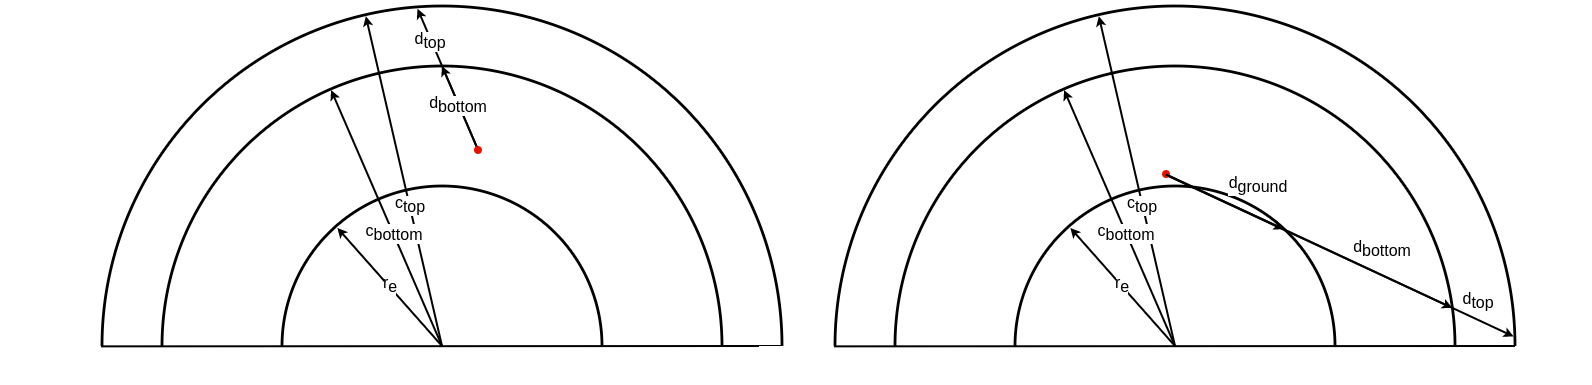
\includegraphics[width=1.0\textwidth]{media/Ground_cloud_intersections.png}
        \caption[Ray intersection situations]{Overview of two situations which can arise when figuring ray intersections
            with cloud layer. $r_{e}$ is the planet radius, $c_{top}$ and $c_{bottom}$ are the
            top and bottom of cloud layer. $d_{ground}$, $d_{bottom}$ and $d_{top}$ are the 
            intersections with planet ground, start of the cloud layer and end of the cloud layer.}
        \label{fig:Cloud layer intersections}
\end{figure}

After this we offset the position of the camera by the distance towards the cloud layer along the
viewing ray and start ray marching. The samples are distributed linearly through the medium, so we use
the \verb|raymarch(...)| function for this purpose. 

To estimate the amount of light reaching each sampled position, we need to perform a secondary 
ray march towards the Sun. We use only a small number of samples for this purpose because the computation
complexity increases very quickly with increasing numbers of secondary samples. The light reaching
each sample is then attenuated by the transmittance accumulated along the ray towards the 
ray origin and the atmosphere transmittance towards the sun stored in Transmittance LUT.   

\begin{figure}
        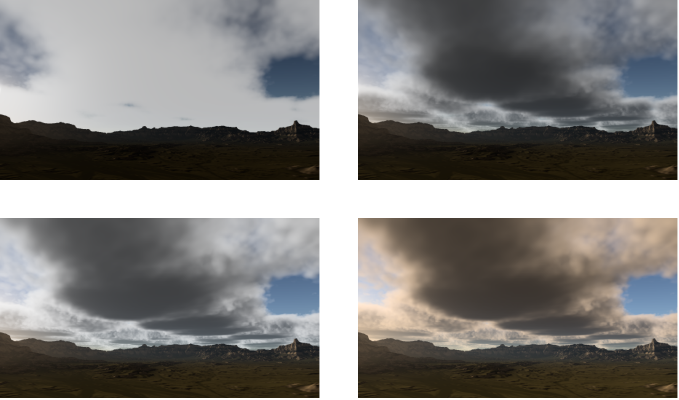
\includegraphics[width=1.0\textwidth]{media/cloud_raymarch_effects.png}
        \caption[Raymarch component effects]{The effect of different components when ray marching clouds. Top left: no secondary ray march toward sun
        Top right: with secondary ray march towards sun Bottom left: secondary ray march to sun and powder
        effect Bottom Right: secondary ray march, powder effect and atmosphere transmittance}
        \label{fig:Cloud Raymarch effects}
\end{figure}

An additional improvement suggested by~\cite{schneider2015real} is to use an additional 
\textit{Powder effect factor} when calculating the transmittance. This effect modifies our 
approximation slightly. With increasing depth inside a cloud, the probability of light 
inscattering in the ray direction increases. To model this increase, we multiply our transmittance
calculated by an additional \textit{Powder effect factor} calculated as follows $P = 1 - e^{-2 \tau}$
where $\tau$ is the optical depth. The effects of the adding the powder effect can be observed in 
Figures~\ref{fig:Cloud Raymarch effects} and~\ref{fig:Powder effect graph}.

\begin{figure}
        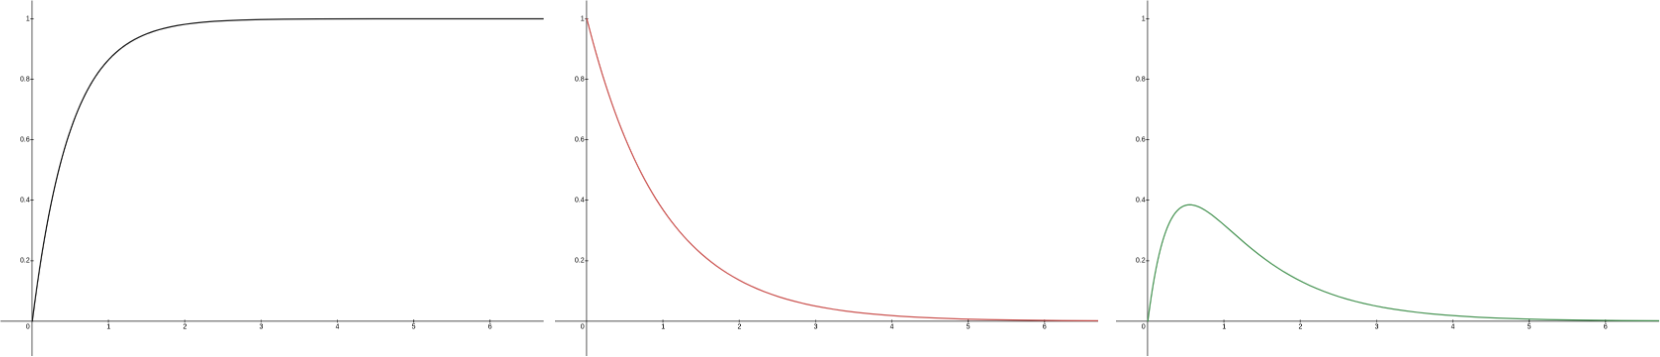
\includegraphics[width=1.0\textwidth]{media/Powder_effect.png}
        \caption[Transmittance calculation curves]{From left to right: (1) Classic transmittance calculation $T = e^{-\tau}$ 
            (2) Powder effect calculation $P = e^{-2 \tau}$ (3) (1) and (2) combined.}
        \label{fig:Powder effect graph}
\end{figure}

The only thing that changes throughout the cloud layer is the cloud density. We use two 3D Worley noise 
textures to simulate the changes in density throughout the medium. During raymarching, we sample 
these textures and multiply their value by the absorption coefficient. First we sample
the higher resolution texture. This texture is used to generate the base low detail shape
of the cloud. After this we sample the smaller texture and subtract it's value from the base
texture producing detailed shapes of the cloud. Before subtracting, we weigh the detailed density
by the inverse of the base density. This results in the detail being subtracted near the edges of the cloud, which is what we want.

\begin{figure}
        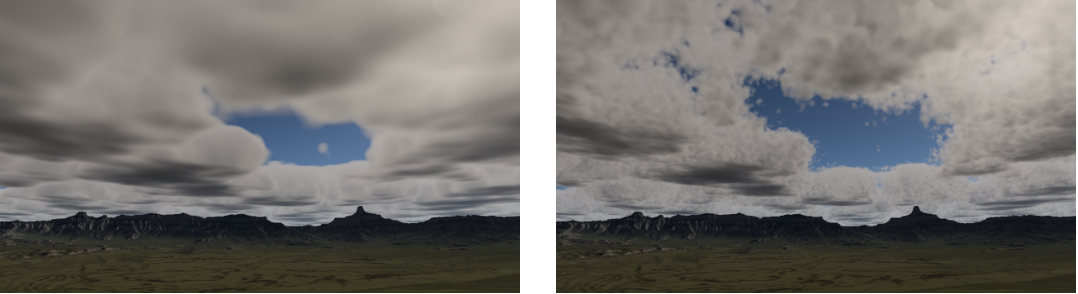
\includegraphics[width=1.0\textwidth]{media/Cloud_baseshape_detailshape.png}
        \caption[Base vs detailed cloud shape]{Left: Only the base shape sampled using the high resolution texture 
                 Right: Detail texture subtracted from the base shape}
        \label{fig:Base shape vs detailed shape}
\end{figure}

As already mentioned, in order to later correctly apply the aerial perspective effects on top of
our clouds, we need to store write the cloud depth into attached depth buffer. We tried three 
different methods to calculate the depth of the cloud. Our first naive attempt was to simply store the 
depth of the first sample, which had transmittance less than a certain threshold. However, we found
that this produced visible bands around the clouds. The resulting depth texture was also very
blocky and did not capture the cloud details well. We then tried the solution proposed by~\cite{hillaire2016physically}.
We store the depth of each sample weighed by the transmittance towards the view point. This is expressed
by the following equation:
\begin{equation}
    C_{depth} = \frac{\sum_{s=0}^{S} T(x_{0},s) * Depth(s)}{\sum_{0}^{S} T(x_{0},s)}
\end{equation}
Where $S$ is the amount of our samples, $s$ is the sampled position, $x_{0}$ is the origin of the view point,
and $(Depth(s))$ is the depth of the respective sample. This resulted in a much more detailed depth texture,
but did not solve the visible outlines. To remove the visible outlines, we linearly 
interpolate the maximum depth with the cloud depth based on the square of the final transmittance from the view 
position towards the final sampled position during our ray march. By doing this, we effectively 
blend the edges of the cloud with the far sky, producing smooth edges. The three depth textures
and the resulting clouds can be seen in Figure~\ref{fig:Cloud depths}  

\begin{figure}
        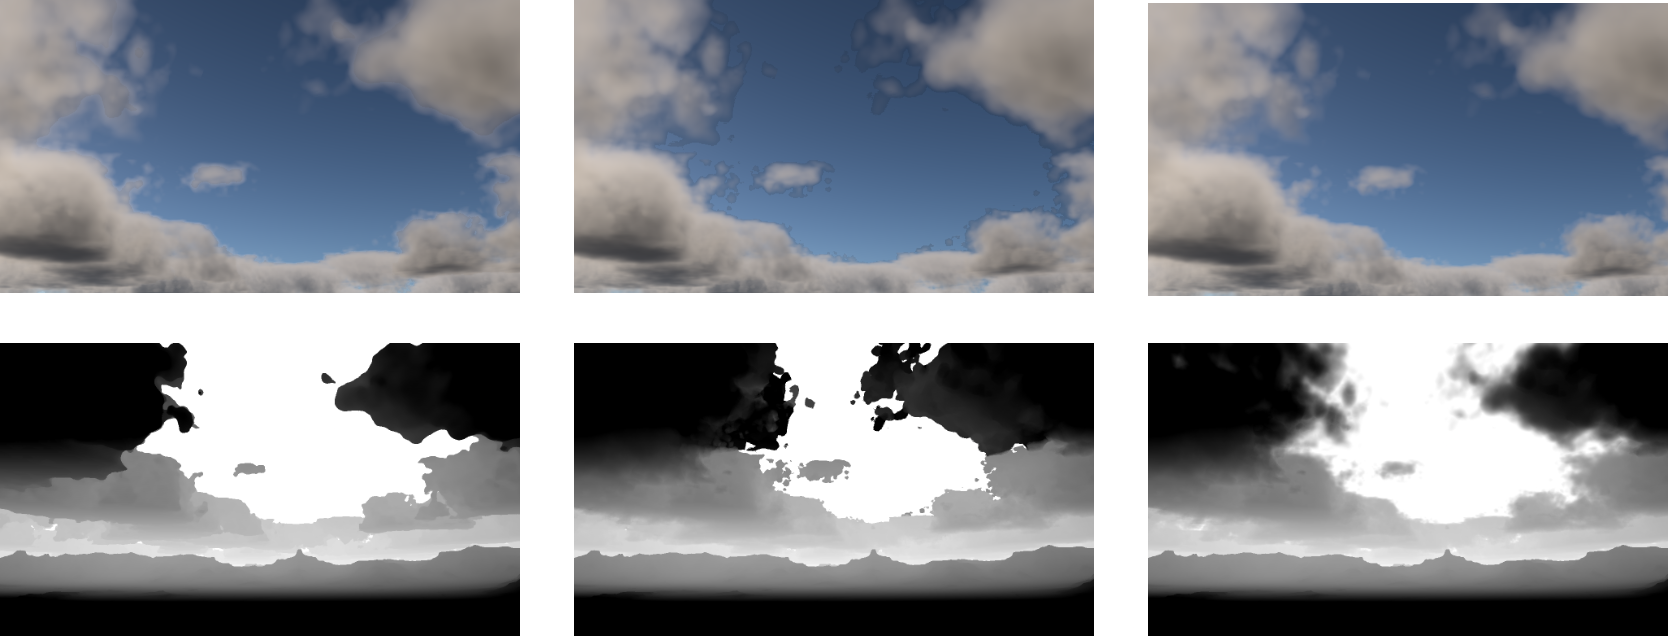
\includegraphics[width=1.0\textwidth]{media/Cloud_depths.png}
        \caption[Cloud depth computation]{From left to right (1) Naive approach storing depth after some transmittance threshold
            (2) Storing depth as sample depth weighed by sample transmittance (3) Storing weighed depth
            and blending edges of clouds}
        \label{fig:Cloud depths}
\end{figure}

The final cloud color is then stored in the RGB channels. The alpha channel contains the final 
transmittance of the cloud. The clouds are then blended with the HDR backbuffer using the following 
equation:
\begin{equation}
    Final Color = BackgroundColor\ *\ CloudColor.A\ +\ CloudColor.RGB
\end{equation}

\subsubsection{Aerial Perspective}
As a last step of the rendering process aerial perspective effects are applied to the entire
scene. Since the Aerial perspective LUT is mapped to the camera frustum, we can use screen 
space coordinates which are the same as the Aerial perspective LUT coordinates. The only thing left
to figure out is which layer we need to sample. We again use the method described previously
in~\ref{lst:Screen to World}. By changing the NDC z value to the depth sampled from depth map 
written by Clouds pass, we get the real-world depth for the processed fragment.

This is then used to sample the Aerial perspective LUT and output it's value. Please note
that we used the alpha channel to store the average transmittance. The blending equation
used by this stage is given by the following equation:
\begin{equation}
    Final Color = BackgroundColor\ * (1.0\ -\ AELUT.A)\ +\ AELUT.RGB 
\end{equation}

\subsection{Post process Histogram and average luminance}
The last stage before we present the image to the screen is the Post processing pass. 
As described above, we use two compute shaders to generate the average luminance, which 
is then used during tonemapping. We use the solution proposed by~\cite{tardif_2019}.

The histogram is represented as a global array with the number of elements equal
to the number of histogram values we want to store. We used the same size as proposed in the reference,
dividing the luminance range into 256 segments. We utilized a local team of threads in a 16x16 block.
Each thread reads a single value stored in the HDR image corresponding to the thread's global dispatch
ID and converts it into luminance. The binary logarithm of this luminance value is then used to 
get the index of the corresponding segment in the histogram. We use a group local histogram copy
to first accumulate all the values. Finally, we merge all local histograms into one single global
histogram.

\begin{lstlisting}[ 
    caption= Code used to generate luminance histogram,
    language=GLSL,
    escapechar=\%,
    label={lst:creating histogram}
]

shared uint HistogramLocal[256];
void main()
{
    vec3 hdrColor = texture(HDRBackbuffer, uv).rgb;
    uint binIndex = HDRToHistogramBin(hdrCol);
    atomicAdd(HistogramLocal[binIndex], 1);

    // wait for all threads in the group to finish 
    // writing into local histogram
    groupMemoryBarrier();
    barrier();

    atomicAdd(HistogramGlobal[gl_LocalInvocationIndex],
              HistogramLocal[gl_LocalInvocationIndex]);
}
\end{lstlisting}

During the second pass, we calculate the weighed sum of all the histogram entries, which is then converted into 
the average luminance for the current image. To calculate the sum, we use the same thread based merge which 
was used when merging Multiscattering LUT values~\ref{lst:multiscattering merge}. By subtracting this new
average luminance from the previously known value, we get the average luminance change between two frames.
We then use the luminance change to slightly offset our old average luminance value. By only offsetting 
the old value instead of overwriting it, we achieve two effects. First, we avoid any artifacts when quickly 
changing scene luminance. Second, this approximates the effect of the eye slowly adapting to increasing (or 
decreasing) light intensity. This effect can be observed in Figure~\ref{fig:Eye luminance adaptation}.

\begin{figure}
        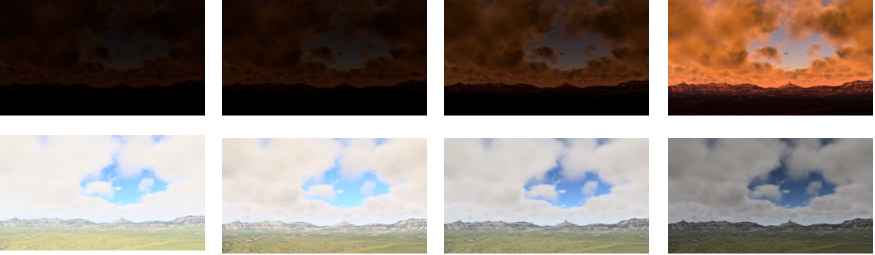
\includegraphics[width=1.0\textwidth]{media/Adaptive_lum_demonstration.png}
        \caption[Adaptive luminance effect]{In the top row we can the adaption effect when the scene suddenly becomes 
            darker. In the bottom the opposite is happening the scene suddenly became overly 
            brighter.}
        \label{fig:Eye luminance adaptation}
\end{figure}

\begin{figure}
        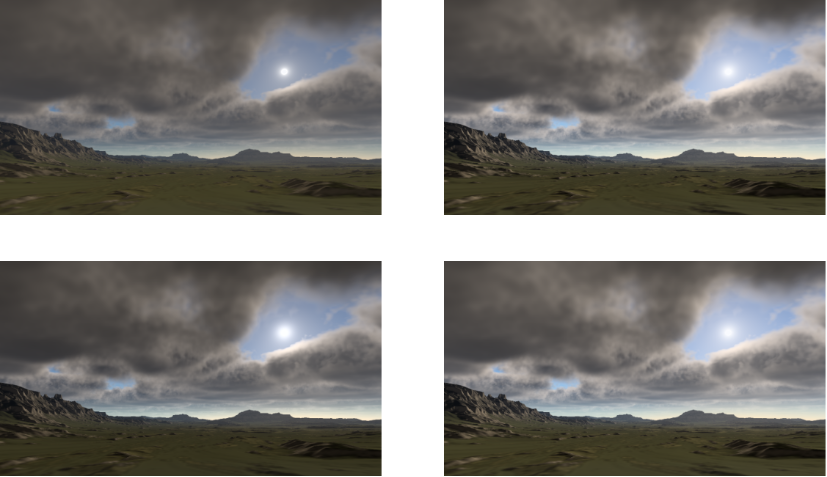
\includegraphics[width=1.0\textwidth]{media/Tonemapping_effects.png}
        \caption[Tonemapping curves comparison]{The effects of different tonemapping curves.
            Top Left: Reinhard Top Right: ACES Bottom Left: Lottes Bottom Right: Uchimura}
        \label{fig:Tonemapping Curves}
\end{figure}

Lastly, the tonemapping shader is executed. The color value stored in the HDR backbuffer is 
converted from RGB space to xyY. Then it is remapped using the average luminance value computed 
previously and transformed using the tonemapping curve. We decided to expose
four tonemapping curves 1. Reinhard tonemapping curve, 2. ACES Filmic Tone mapping curve~\cite{narkowicz2016aces}
3. Lottes tonemapping curve~\cite{lottes2016} and 4. Uchimmura tonemapping curve~\cite{uchimura2018practical} 
used in Gran Turismo. The comparison of these curves can be seen in Figure~\ref{fig:Tonemapping Curves}.

\chapter{Results}
In this chapter, we present the results we obtained using our implementation.
We also compare the performance of each scene on two different computers with the parameters provided in Table~\ref{tab:Pc Specs}.
Most of our frame budget was spent on raymarching clouds. Performance is highly dependent on the 
resulting cloud quality we want to achieve. In all of our benchmarks, we only had a single
frame in flight. This slightly reduces the stability of the frame rate, but in return gives more consistent measurements.


\begin{center}
\begin{table}[h]
\begin{tabular}{ ||c|c|c|c|| } 
\hline
Name & Type  & CPU & GPU \\
\hline
PC1 & Desktop & AMD RYZEN 7 1700 & GeForce GTX 1080 \\
\hline
PC2 & Laptop & Intel Core i7 7700HQ & GeForce GTX 1050 (mobile)\\
\hline
\end{tabular}
\caption[PC specs]{\label{tab:Pc Specs} Computers and their hardware components performance was tested on.}
\end{table}
\end{center}

\section{Earth with no cloud cover}
In the first scene, we would like to compare the look of the atmosphere without any cloud cover with real photos to 
see how accurate our model is. The scattering and extinction coefficients of the atmosphere used for this purpose can be seen 
in Table~\ref{tab:Earth Coeff}. We would also like to compare the aerial perspective effects of the atmosphere onto 
opaque objects. Multiple pairs of images will follow, each containing our rendered image and a real photo. 

In Figure~\ref{fig:Atmosphere sunset comparison} we can see the comparison of sunset images. We can see that the 
overall palette is the same; however, slight changes are still present. The most striking difference is the 
lighting of the hills. Because we sample directly Transmittance LUT towards the Sun at each terrain fragment when 
the sun is behind the horizon, we get completely black terrain, which is not correct.

Figure~\ref{fig:Atmosphere sunset comparison} shows another comparison between the photo and the image rendered by our application.
We can again see that ours has a similar color composition, but it is a bit darker. This could be caused by the manual settings
of the camera used to shoot the real photo versus our automatic adaptive luminance balancing.


Last Figure~\ref{fig:Atmosphere day comparison} shows comparison between photo and rendered image of clear day.
Similarly to the previous comparison, our application produces a sky that looks darker. Along with this, the aerial perspective
effects of the atmosphere can be clearly visible making the mountains look bluish white.

\begin{center}
\begin{table}[h]
\begin{tabular}{ ||c|c|c|c|| } 
\hline
Coefficient & Value ($km^{-1}$) & Distribution \\
\hline
\hline
$\beta^{scat}_{R}$ & (5.802 $\cdot\ 10^{-3}$,\ 13.558 $\cdot\ 10^{-3}$,\ 33.100 $\cdot\ 10^{-3}$) & $e^{\frac{-h}{8.0}}$ \\
\hline                                                                          
$\beta^{scat}_{M}$ & (3.996 $\cdot\ 10^{-3}$,\ 3.996  $\cdot\ 10^{-3}$,\ 3.996  $\cdot\ 10^{-3}$) & $e^{\frac{-h}{1.2}}$ \\
\hline                                                                          
$\beta^{ext}_{M}$ & (4.440  $\cdot\ 10^{-3}$,\ 4.440  $\cdot\ 10^{-3}$,\ 4.440  $\cdot\ 10^{-3}$) & $e^{\frac{-h}{1.2}}$ \\
\hline
\multirow{2}{*}{$\beta^{ext}_{O}$} & \multirow{2}{*}{(0.650 $\cdot\ 10^{-3}$,\ 1.881 $\cdot\ 10^{-3}$,\ 0.085 $\cdot\ 10^{-3}$)} & (h < 25 km) $\frac{h}{15} - \frac{2}{3}$ \\
& & (h > 25 km) $\frac{8}{3}-\frac{h}{15}$ \\
\hline
\end{tabular}
\caption[Earth-like coefficients]{\label{tab:Earth Coeff} Coefficients used to simulate atmosphere.}
\end{table}
\end{center}

\begin{figure}[h]
    \centering
    \begin{subfigure}[b]{0.49\textwidth}
        \centering
        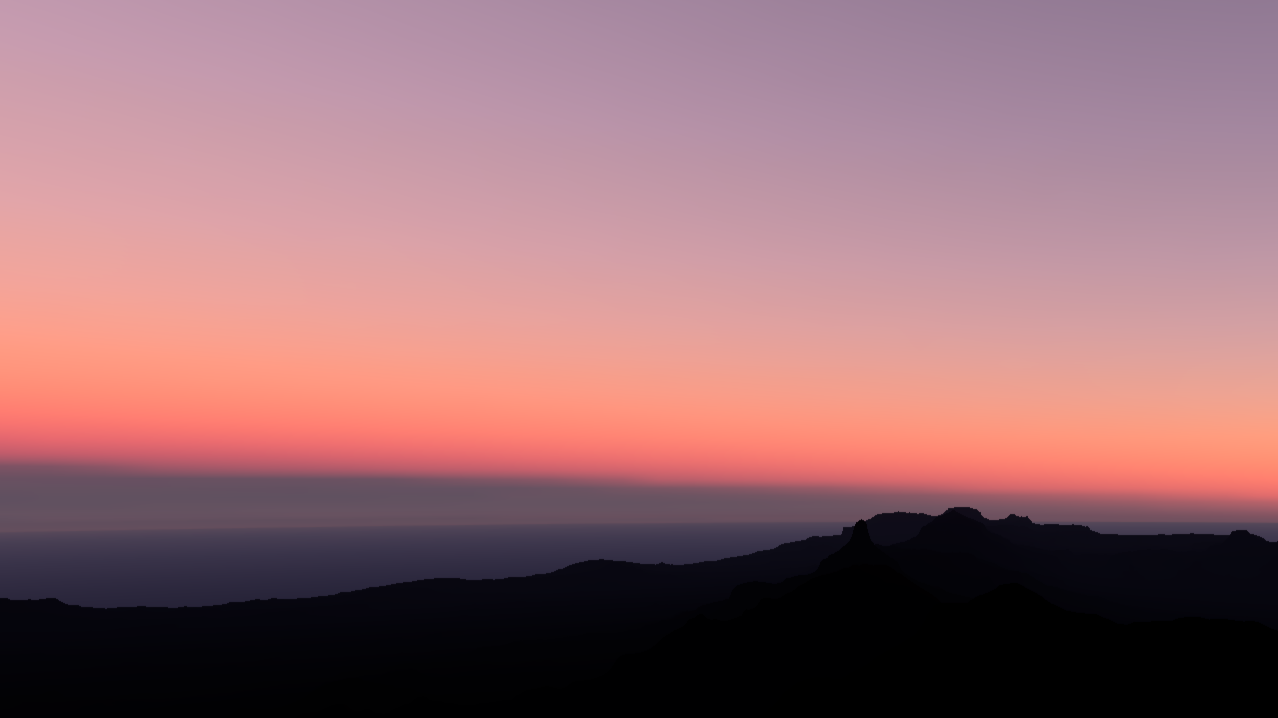
\includegraphics[width=\textwidth]{media/atmosphere_sunset.png}
        \caption{Image rendered by our application.}
        \label{fig:Render of sunset}
    \end{subfigure}
    \hfill
    \begin{subfigure}[b]{0.49\textwidth}
        \centering
        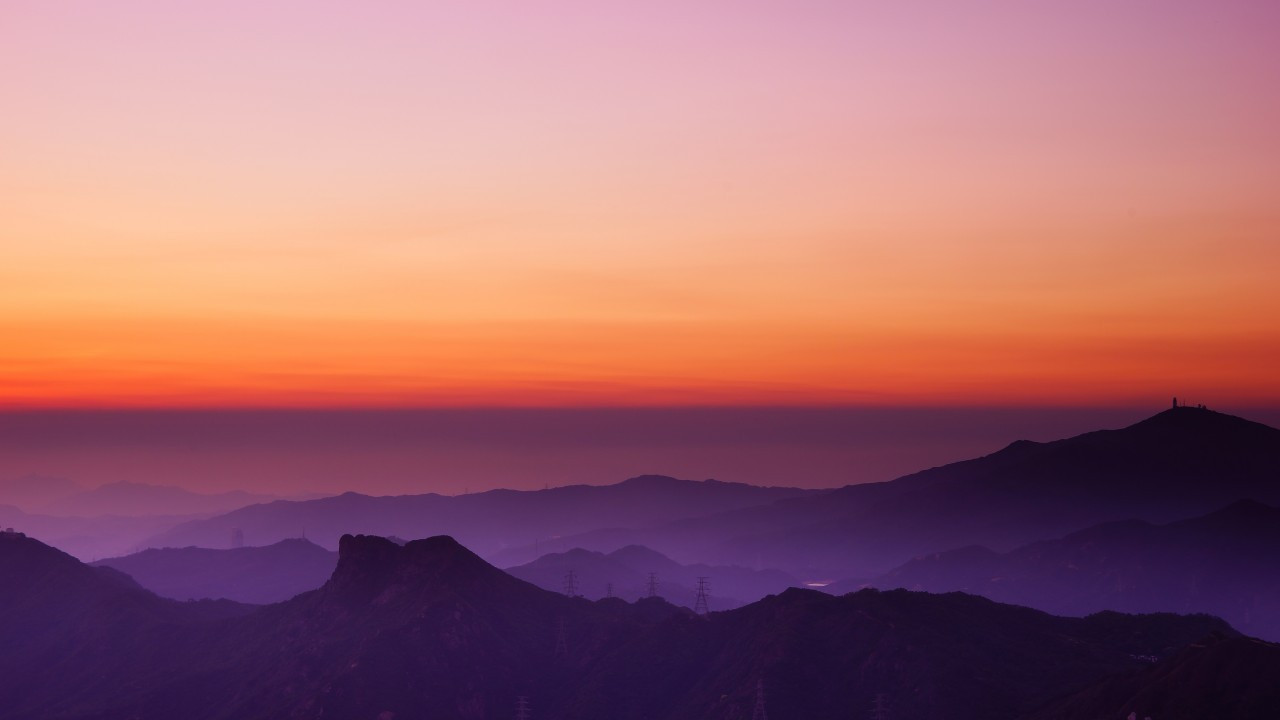
\includegraphics[width=\textwidth]{media/atmosphere_sunset_real.jpeg}
        \caption{Real photo of sunset (source \href{https://www.wallpapermaiden.com/wallpaper/39029/sunset-horizon-mountains-hills-clear-sky/download/1280x720}{Here})}
        \label{fig:Photo of sunset}
    \end{subfigure}
    \caption{Comparison between image rendered by our application and real photo of sunset.}
    \label{fig:Atmosphere sunset comparison}
\end{figure}

\begin{figure}[h]
     \centering
     \begin{subfigure}[b]{0.49\textwidth}
         \centering
         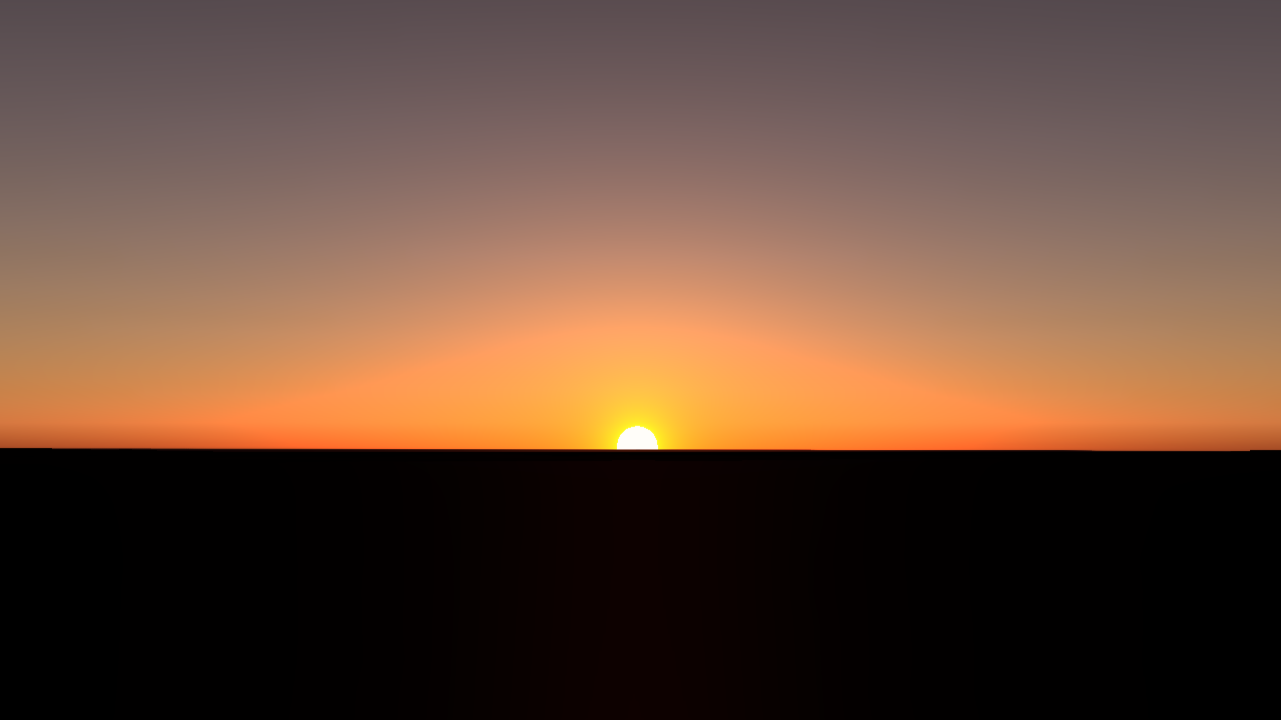
\includegraphics[width=\textwidth]{media/Sunset_atmo_yellow.png}
         \caption{Image rendered by our application.}
         \label{fig:Render of yellow sunset}
     \end{subfigure}
     \hfill
     \begin{subfigure}[b]{0.49\textwidth}
         \centering
         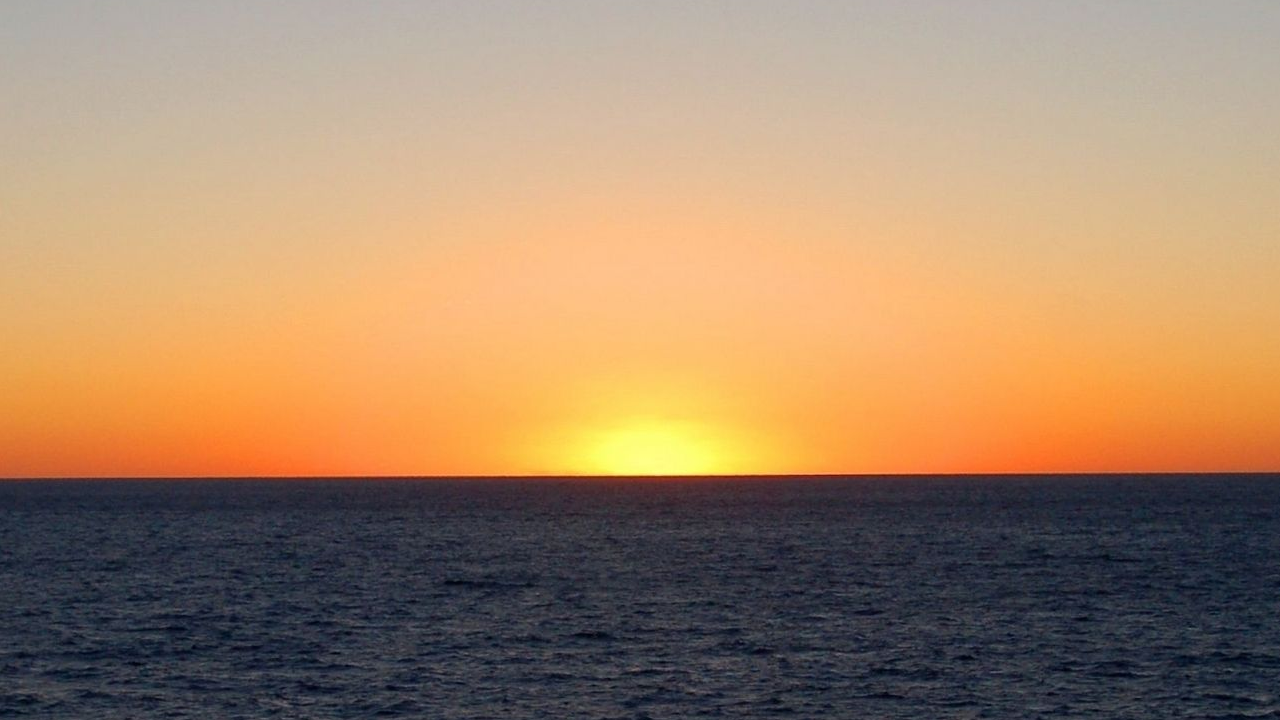
\includegraphics[width=\textwidth]{media/Sunset_atmo_yellow_real.png}
         \caption{Real photo of sunset (source \href{https://wallpaperaccess.com/clear-sunset}{Here})}
         \label{fig:Photo of yellow sunset}
     \end{subfigure}
     \hfill
        \caption{Comparison between image rendered by our application and real photo of sunset.}
        \label{fig:Atmosphere yellow sunset comparison}
\end{figure}

\begin{figure}[h]
     \centering
     \begin{subfigure}[b]{0.49\textwidth}
         \centering
         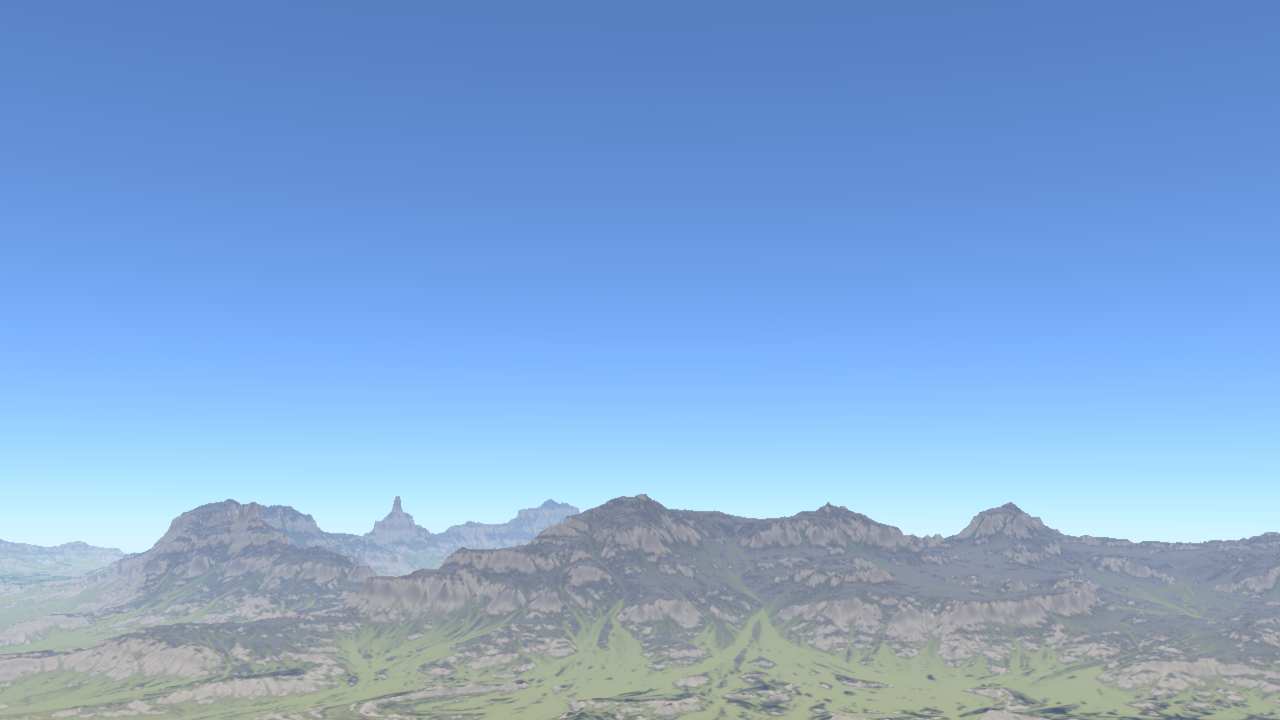
\includegraphics[width=\textwidth]{media/atmosphere_day.png}
         \caption{Rendered image of clear day.}
         \label{fig:Render of atmosphere during day}
     \end{subfigure}
     \hfill
     \begin{subfigure}[b]{0.49\textwidth}
         \centering
         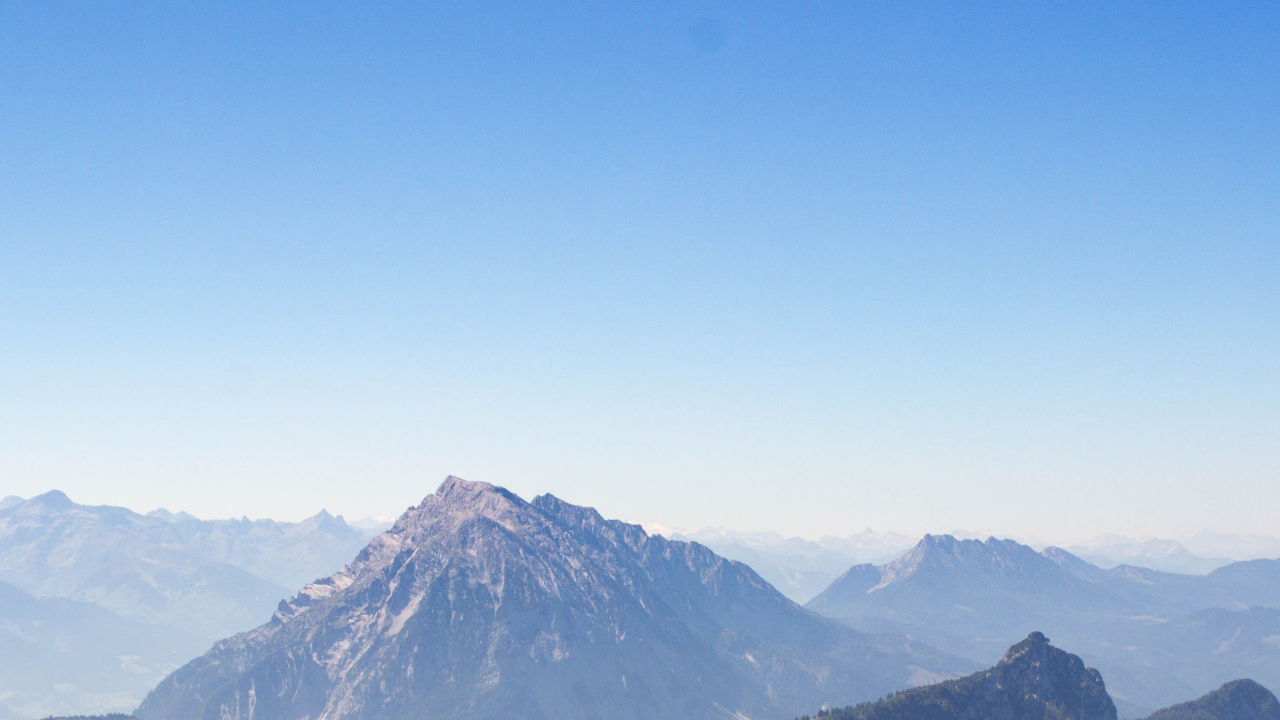
\includegraphics[width=\textwidth]{media/atmosphere_day_real.png}
         \caption{Photo of clear day (source \href{https://wallup.net/preview/?wallpaper=landscape-mountains-clear-sky}{Here}).}
         \label{fig:Photo of atmosphere during day}
     \end{subfigure}
     \hfill
        \caption{Comparison between image rendered by our application and real photo of clear day.}
        \label{fig:Atmosphere day comparison}
\end{figure}

\section{Earth with medium cloud cover}
Second test scene again uses earth like atmosphere setup. The atmosphere scattering and absorption coefficients are the same as in 
the previous scene and can again be seen in Table~\ref{tab:Earth Coeff}. We use a layer of clouds starting at 5.7 kilometers
and ending at 8 kilometers. This is 
a bit higher than one would possibly find Cumulus clouds such as the ones we are trying to depict. We chose to place the clouds
higher to compensate for the scale at which we are trying to display the scene. We can also see the effect of Aerial perspective
in the second and third images when looking at the distant hills. The resulting images can be seen in Figure\ref{fig:Earth-like results} and the performance of
individual shaders in Table~\ref{tab:Earth like performance}. We can see that we are only barely hitting 60 fps on PC1, while
in order to at least get close to 30 fps on PC2, we need to reduce the resolution to 720p.  


Another thing to notice is that the main bottleneck is cloud rendering. It is usually responsible for over 
60\% of the total frame time. The LUT's are not screen resolution dependent; thus the time spent pre-calculating is 
almost the same for both 1080p and 720p.
Additionally, the increase in time spent drawing atmospheric effects (not clouds) is also as decoupled as possible
from the screen resolution. The increased cost when rendering Far Sky and Aerial perspective is only due to the 
increased amount of pixels we need to process and draw the sky texture on. The same holds for the Histogram computation as well
as Tonemaping, because they also iterate over the whole screen.

\begin{center}
\begin{table}[h]
\begin{tabular}{ ||c|c|c|c|c|| } 
\hline
& \multicolumn{2}{|c|}{PC1} & \multicolumn{2}{|c||}{PC2} \\
\hline
Shader              & 1080p          & 720p         &1080p         &  720p           \\
\hline
Transmittance LUT   & 63.9 $\mu s$   & 63.9 $\mu s$ & 233.7 $\mu s$&  235.4 $\mu s$  \\
\hline
Multiscattering LUT & 51.0 $\mu s$   & 51.1 $\mu s$ & 208.4 $\mu s$&  210.0 $\mu s$  \\
\hline
Sky View LUT        & 33.3 $\mu s$   & 32.4 $\mu s$ & 129.7 $\mu s$&  130.6 $\mu s$  \\
\hline
AE Perspective LUT  & 56.2 $\mu s$   & 56.4 $\mu s$ & 184.9 $\mu s$&  186.5 $\mu s$  \\
\hline
\hline
Draw Terrain        & 2.9 $ms$       & 2.9 $ms$     & 10.86 $ms$   &  11.73 $ms$     \\
\hline
Draw Far Sky        & 216.7 $\mu s$  & 104.7 $\mu s$& 979.9 $\mu s$&  384.6 $\mu s$  \\
\hline
Draw Clouds         & 11.6 $ms$      & 7.15 $ms$    & 43.7 $ms$    &  22.85 $ms$     \\
\hline
Draw AE Perspective & 278.3 $\mu s$  & 125.9 $\mu s$& 1.26 $ms$    &  569.7 $\mu s$  \\
\hline
\hline
Construct Histogram & 228.1 $\mu s$  & 103.6 $\mu s$& 415.3 $\mu s$&  187.9 $\mu s$  \\
\hline
Sum Histogram       & 3.3 $\mu s$    & 3.3 $\mu s$  & 3.9 $\mu s$  &  3.7 $\mu s$    \\
\hline
Tonemap             & 341.0 $\mu s$  & 147.3 $\mu s$& 1.12 $ms$    &  500.0 $\mu s$  \\
\hline
\hline
Total              & 15.79 $ms $     & 10.73 $ms$   & 59.1 $ms$    &   36.99 $ms$    \\
\hline
\end{tabular}
\caption[Earth-like planet performance]{\label{tab:Earth like performance} Average execution times of each shader
    for earth like planet with clouds.}
\end{table}
\end{center}

\pagebreak

\begin{figure}[h!]
     \centering
     \begin{subfigure}[b]{1.0\textwidth}
         \centering
         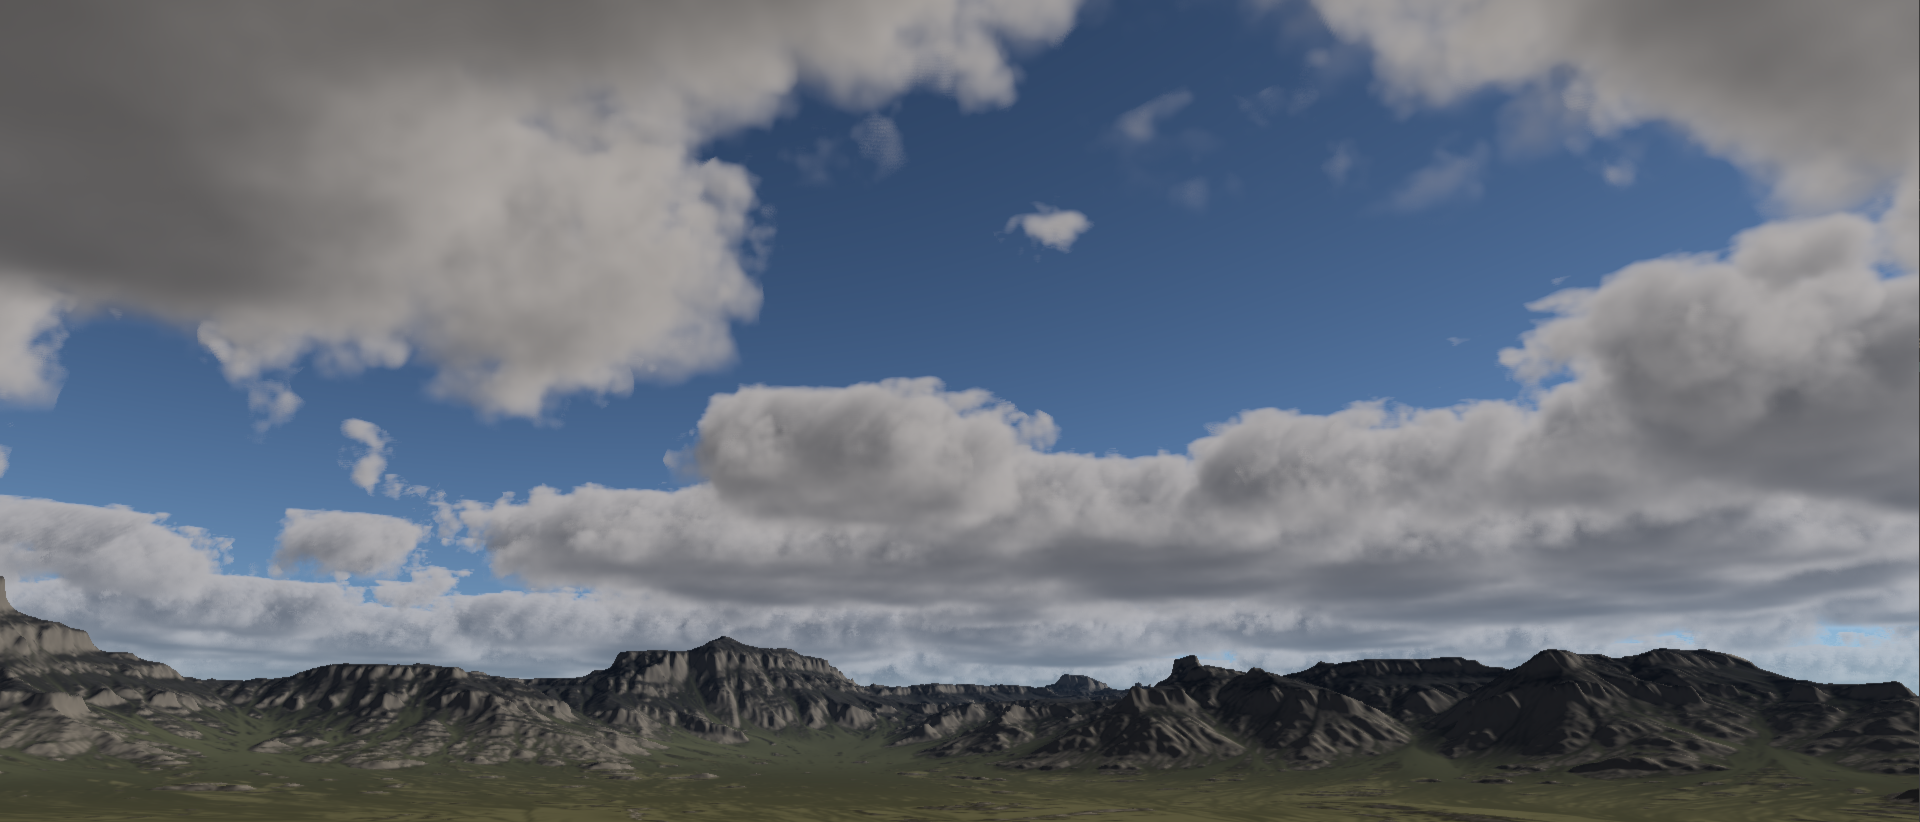
\includegraphics[width=\textwidth]{media/Earth_like_result_1.png}
         \caption{Medium cloud cover with sun almost directly overhead.}
         \label{fig:Earth-like medium cloud cover}
     \end{subfigure}
     \quad
     \begin{subfigure}[b]{1.0\textwidth}
         \centering
         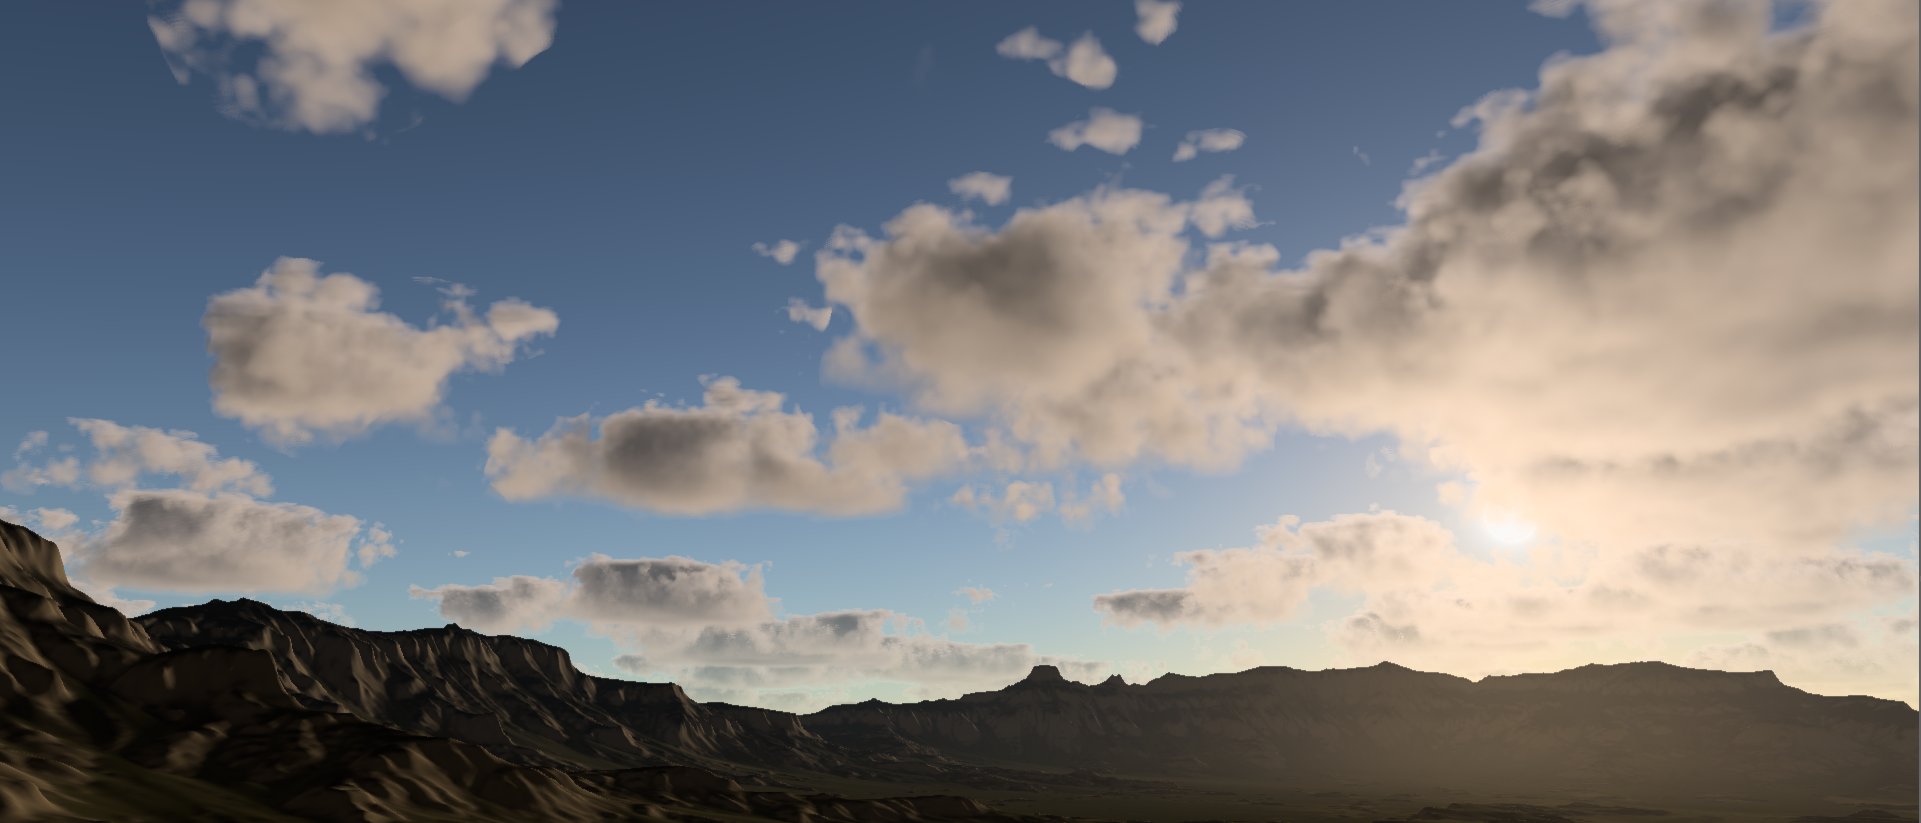
\includegraphics[width=\textwidth]{media/Earth_like_result_2.png}
         \caption{Sparse cloud cover with sun nearing sunset. Aerial perspective 
         effects are clearly visible on the terrain towards the sun.}
         \label{fig:Earth-like sparse cloud cover}
     \end{subfigure}
     \quad
     \begin{subfigure}[b]{1.0\textwidth}
         \centering
         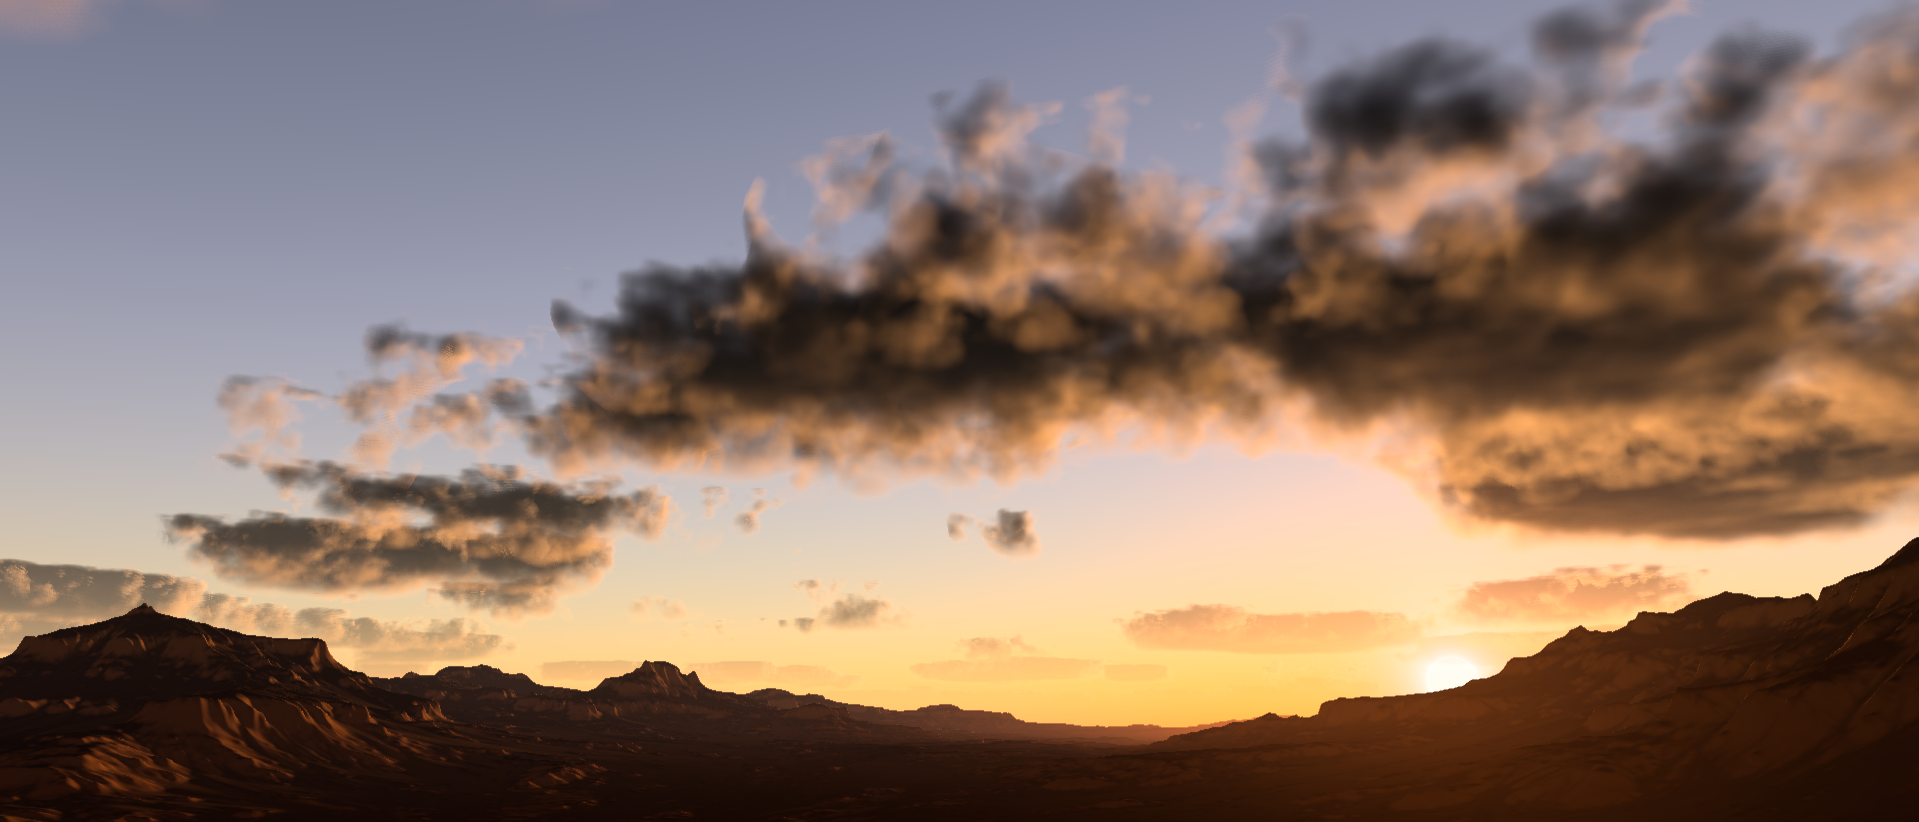
\includegraphics[width=\textwidth]{media/Earth_like_result_3.png}
         \caption{Clouds during sunset. The clouds become lot darker as not a lot of sunlight
         reaches them through the atmosphere. }
         \label{fig:Earth-like sunset}
     \end{subfigure}
        \caption[Earth-like results with clear weather]{Images of clouds and atmosphere obtained by using Earth-like conditions.}
        \label{fig:Earth-like results}
\end{figure}

\section{Fictional Planet}
Last scene uses cloud and atmosphere parameters that are not based in reality. These settings are used to demonstrate
the flexibility of our implementation. Given the procedural nature of our clouds combined with the parameterizable atmosphere,
we are able to completely change the overall look and mood of the entire scene by tweaking a few values. Additionally, 
these fictional settings demonstrate the interconnected effects of both atmosphere and clouds producing 
consistent results even when we change the values outside of the ranges we are able to observe in the real world. The atmospheric
parameters used to render this scene can be seen in Table~\ref{tab:Fictional Coeff}. 

We have raised the Mie scattering and extinction coefficients, as well as the Rayleigh scattering coefficient, by almost two orders. 
Together with the increase in the distribution of particles throughout the medium, we are able to simulate a very dense
atmosphere. We achieved the purplish blue look of the atmosphere by leaving the blue-wavelength component of the Rayleigh
scattering coefficient lower. As a result, most of the light in the red-green wavelength gets scattered away by the atmosphere
before reaching the eye of the observer. To match the aerial perspective effects with the sky look, we also lowered the 
blue-wavelength component of the Mie absorption coefficient, allowing more blue light to penetrate the atmosphere.

\begin{center}
\begin{table}[h]
\begin{tabular}{ ||c|c|c|c|| } 
\hline
Coefficient & Value ($km^{-1}$) & Distribution \\
\hline
\hline
$\beta^{scat}_{R}$ & (0.149,\ 0.142,\ 0.051) & $e^{\frac{-h}{18.416}}$ \\
\hline
$\beta^{scat}_{M}$ & (0.046,\ 0.047,\ 0.057) & $e^{\frac{-h}{13.143}}$ \\
\hline
$\beta^{ext}_{M}$ & (0.082 ,\ 0.071,\ 0.058) & $e^{\frac{-h}{13.143}}$ \\
\hline
\multirow{2}{*}{$\beta^{ext}_{O}$} & \multirow{2}{*}{(0.650 $\cdot\ 10^{-3}$,\ 1.881 $\cdot\ 10^{-3}$,\ 0.085 $\cdot\ 10^{-3}$)} & (h < 25 km) $\frac{h}{15} - \frac{2}{3}$ \\
& & (h > 25 km) $\frac{8}{3}-\frac{h}{15}$ \\
\hline
\end{tabular}
\caption[Fictional coefficients]{\label{tab:Fictional Coeff} Coefficients used to simulate the atmosphere on a fictional planet.}
\end{table}
\end{center}

Similarly to the previous scenes, the performance can be observed in Table~\ref{tab:Fictional performance}. Most of the results
stay the same with the one big exception of clouds. By raising the density of the clouds in the fictional scene, we are able 
to greatly reduce the number of raymarching samples used for each cloud. This is due to the cloud shader terminating the 
raymarch earlier when a certain accumulated density threshold was reached. We are able to do this because for very high
accumulated densities the amount of light increase with each additional sample is negligible and thus has almost no visual
impact on the final result.

These optimizations can also introduce artifacts, resulting in visually unappealing results whenever we increase the 
cloud density too much. In the case of this scene it was possible to raise
the cloud density quite high because the dense atmosphere hides away most of the imperfections produced.


\begin{center}
\begin{table}[h]
\begin{tabular}{ ||c|c|c|c|c|| } 
\hline
& \multicolumn{2}{|c|}{PC1} & \multicolumn{2}{|c||}{PC2} \\
\hline
Shader              & 1080p          & 720p         &1080p         &  720p           \\
\hline
Transmittance LUT   & 64.2 $\mu s$   & 63.9 $\mu s$ & 234.8 $\mu s$&  236.6 $\mu s$  \\
\hline
Multiscattering LUT & 51.1 $\mu s$   & 51.2 $\mu s$ & 209.3 $\mu s$&  211.0 $\mu s$  \\
\hline
Sky View LUT        & 32.7 $\mu s$   & 32.3 $\mu s$ & 130.2 $\mu s$&  131.2 $\mu s$  \\
\hline
AE Perspective LUT  & 56.8 $\mu s$   & 56.4 $\mu s$ & 185.8 $\mu s$&  187.2 $\mu s$  \\
\hline
\hline
Draw Terrain        & 2.86 $ms$       & 2.88 $ms$     & 10.31 $ms$   &  10.44 $ms$     \\
\hline
Draw Far Sky        & 216.2 $\mu s$  & 101.6 $\mu s$& 896.1 $\mu s$&  441.6 $\mu s$  \\
\hline
Draw Clouds         & 7.89 $ms$      & 5.13 $ms$    & 22.52 $ms$    &  13.75 $ms$     \\
\hline
Draw AE Perspective & 277.76 $\mu s$  & 125.4 $\mu s$& 1.26 $ms$    &  569.7 $\mu s$  \\
\hline
\hline
Construct Histogram & 227.2 $\mu s$  & 103.0 $\mu s$& 418.0 $\mu s$&  186.1 $\mu s$  \\
\hline
Sum Histogram       & 3.3 $\mu s$    & 3.3 $\mu s$  & 3.8 $\mu s$  &  3.7 $\mu s$    \\
\hline
Tonemap             & 342.3 $\mu s$  & 146.4 $\mu s$& 1.13 $ms$    &  494.0 $\mu s$  \\
\hline
\hline
Total              & 12.02 $ms $     & 8.69 $ms$    & 37.3 $ms$    &   26.96 $ms$    \\
\hline
\end{tabular}
\caption[Fictional planet performance]{\label{tab:Fictional performance} Average execution times of each shader for the fictional planet.}
\end{table}
\end{center}

\begin{figure}[h!]
     \centering
     \begin{subfigure}[b]{1.0\textwidth}
         \centering
         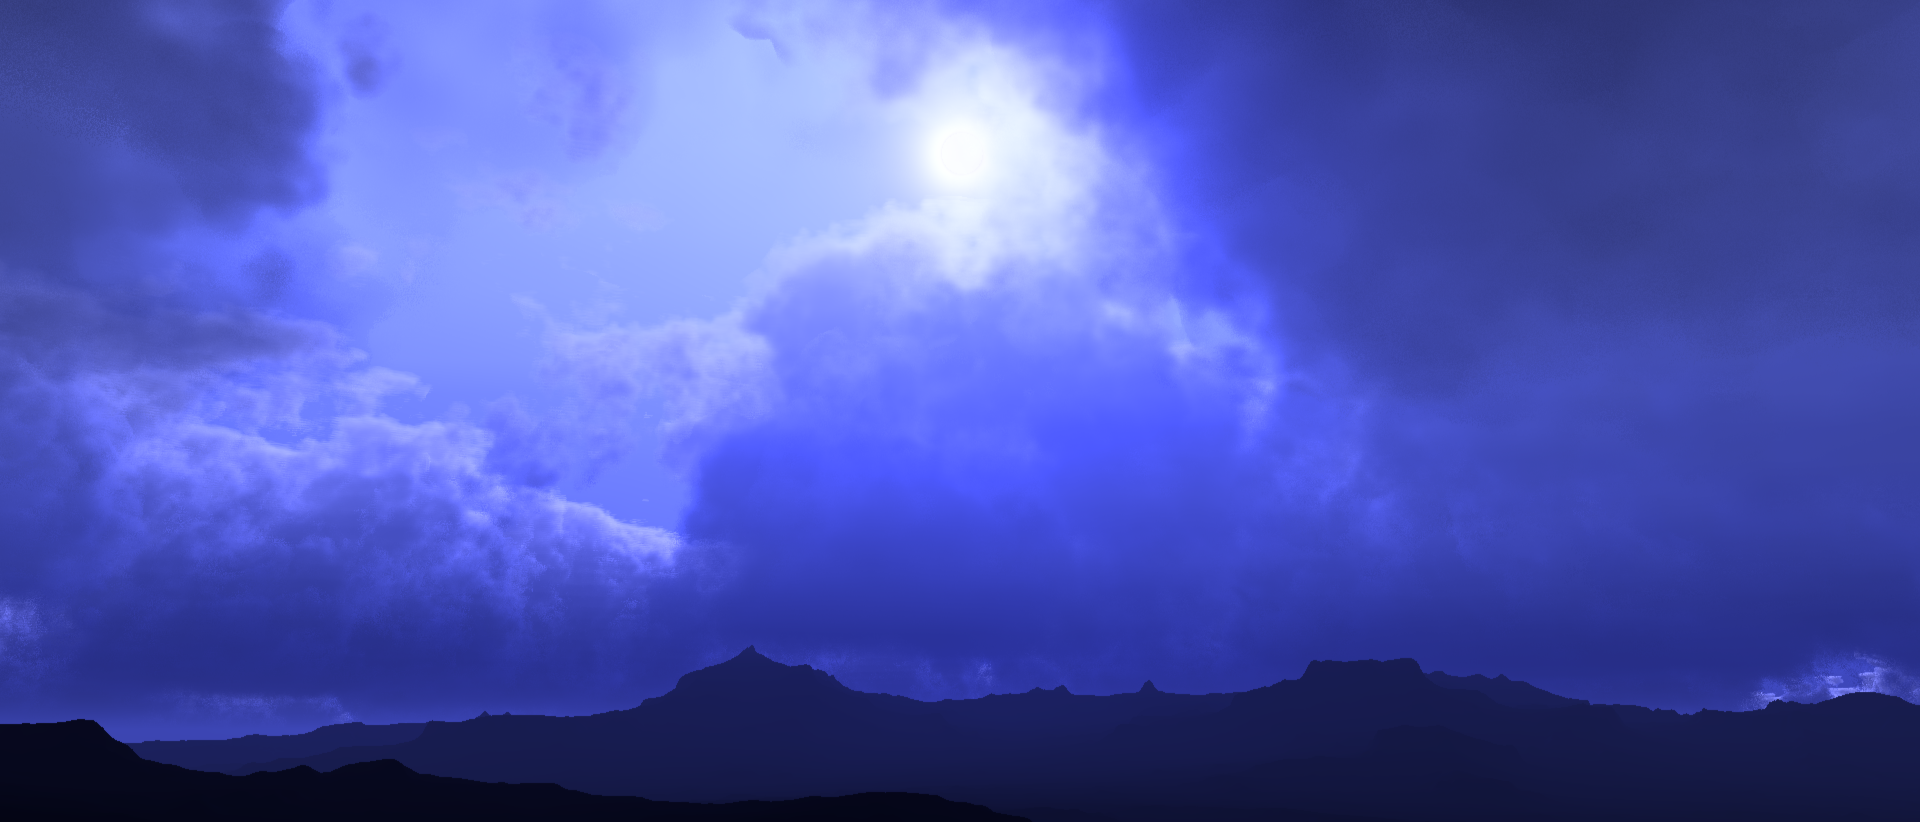
\includegraphics[width=\textwidth]{media/Alien_planet_1.png}
         \caption{Dense cloud cover with big cloud layer.}
         \label{fig:Fictional big cloud layer}
     \end{subfigure}
     \quad
     \begin{subfigure}[b]{1.0\textwidth}
         \centering
         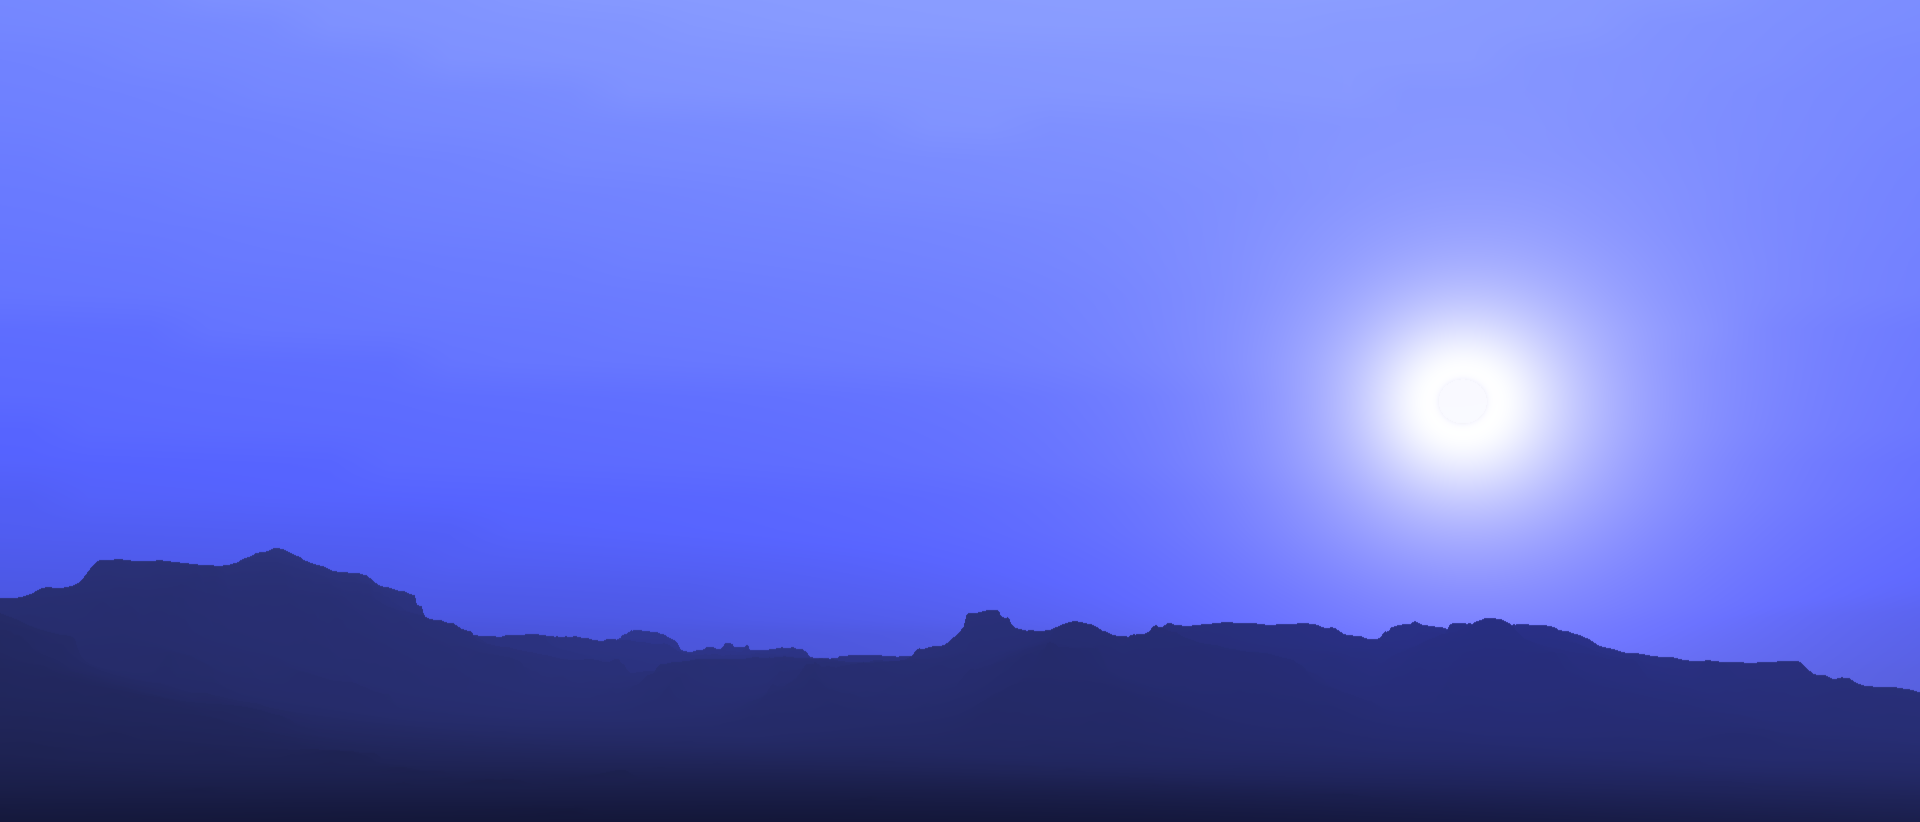
\includegraphics[width=\textwidth]{media/Alien_planet_2.png}
         \caption{Sun is near horizon wihtout any clouds. The blue tinted atmosphere is very clearly visible.}
         \label{fig:Fictional no clouds}
     \end{subfigure}
     \quad
     \begin{subfigure}[b]{1.0\textwidth}
         \centering
         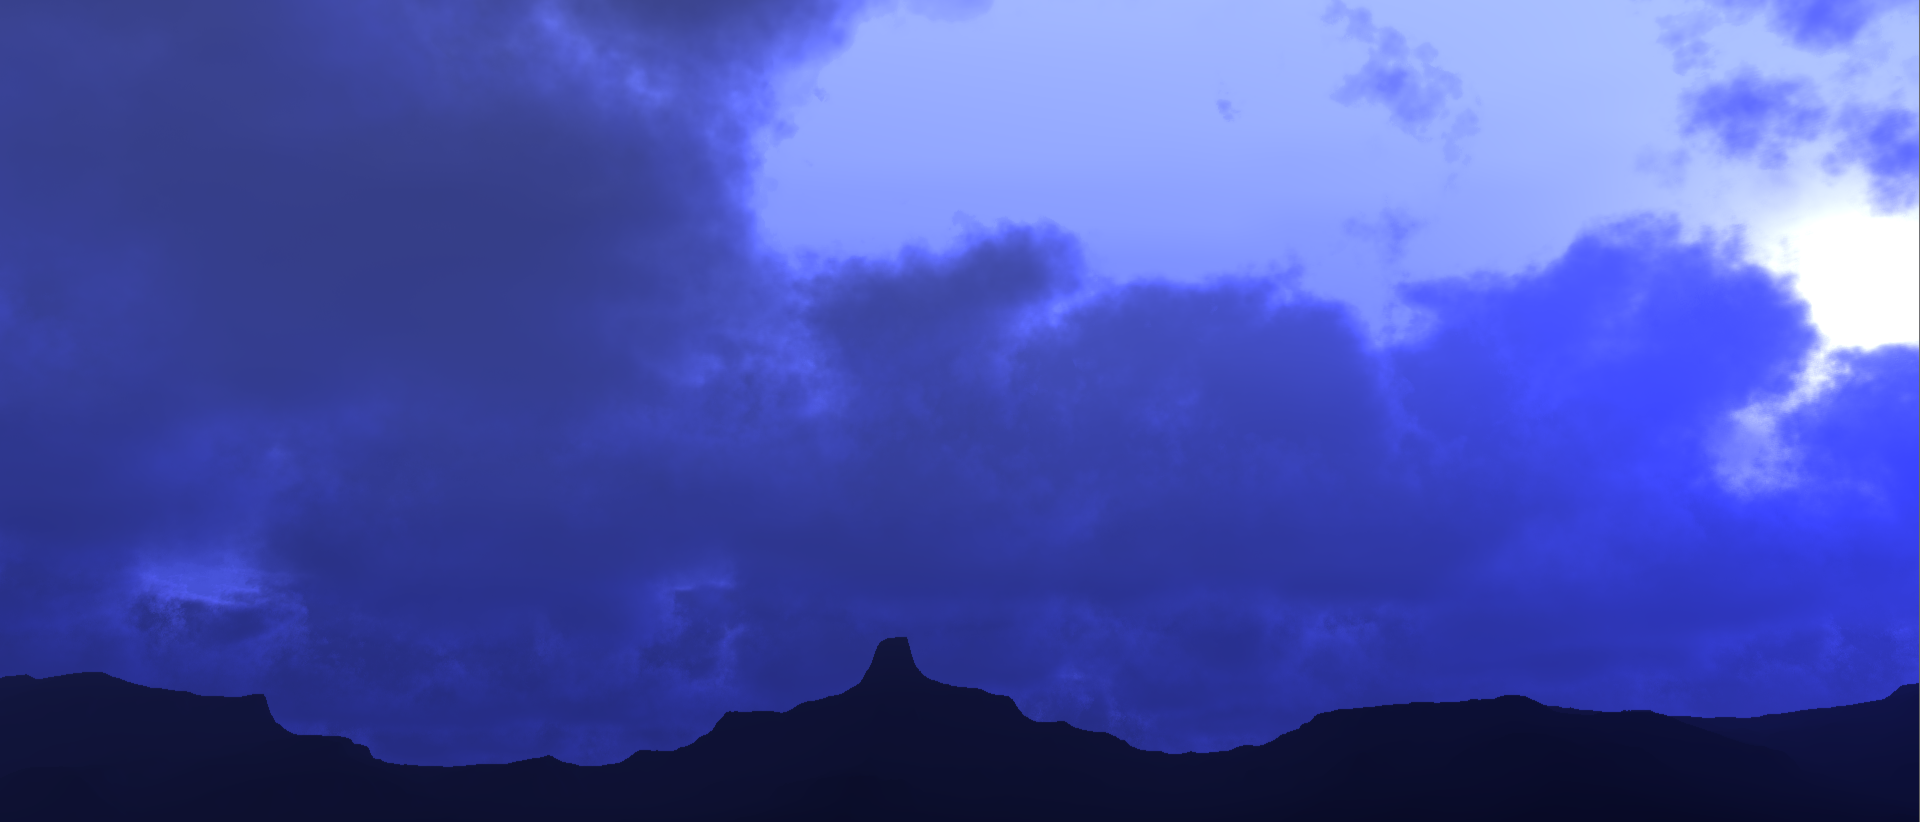
\includegraphics[width=\textwidth]{media/Alien_planet_3.png}
         \caption{Sun is near horizon and clouds are lower than in Figure~\ref{fig:Fictional big cloud layer}. 
            Most of the light is absorbed by the atmosphere before it reaches the cloud layer.}
         \label{fig:Fictional sunset clouds}
     \end{subfigure}
        \caption[Fictional planet]{Images of clouds and atmosphere obtained by using Earth-like conditions.}
        \label{fig:Fictional planet results}
\end{figure}

\chapter{Conclusion}
In this work, we have described the implementation of several techniques combined to create a single 
interconnected system to render atmospheric effects. By using Vulkan API we were successfully able to 
leverage GPU for most of our computations and thus reach real-time frame rates. The model previously described
by Hillaire~\cite{hillaire_2020} was used to render the sky. On top of this, a technique presented by Shneider
~\cite{schneider2015real} was implemented, allowing us to combine the atmosphere model with procedurally generated
clouds. 

The implemented solution allows visualization of miscellaneous settings ranging from those based in reality
all the way to those completely fictional. Although this implementation relies on the use of multiple LUTs, it is 
still possible to change almost all the parameters during the run-time of the application. 

\section{Future work}
The most pressing issue of the implementation presented is the performance of rendering clouds. First, due to the fact
that clouds are raymarched for each pixel of the resulting image, there is a dependency on the resolution of the final 
image. One possible improvement would be to render the clouds into a fixed-sized texture (similarly to how the sky view LUT
texture is generated), which would then be sampled and up-scaled to fit the final resolution. Additionally, we could reduce 
the amount of raymarching needed for each frame by updating only one out of sixteen pixels for each 4x4 block of pixels for
each frame. Combining this by reprojecting the previous frame would keep the visual quality high while significantly reducing
the amount of raymarching done each frame. Secondary benefit of using this approach would be the option to use noise for offsetting
start of each ray at the start of raymarching more aggressively, which would allow us to use fewer samples and reduce the 
raymarch complexity even further.

Another thing missing from our application are shadows. We believe that by adding hard as well as soft volumetric shadows
one could improve the appeal and realism of the resulting images significantly. 

\bibliographystyle{alpha}
\bibliography{thesisbib}

\appendix
\chapter{Building and controlling the application}
\subsection{Building the application}
Our application uses Premake to create a project or makefile which is then used to generate the executable.

When building on Linux, the following dynamic libraries have to be installed: \href{https://www.glfw.org}{glfw}
and \href{https://vulkan.lunarg.com/sdk/home#linux}{vulkan-dll} 

The steps to successfully use the application on Linux are as follows.

\begin{enumerate}
    \item Download and install Vulkan SDK and GLFW.
    \item Go to the root directory and from the command line call \textbf{premake5 gmake}.
    \item From the command line call \textbf{compile\_shaders\_linux.sh}.
    \item From the command line call \textbf{make config$=$debug\_linux}.
    \item Run the executable stored in bin/Linux/Debug/Atmosphere
\end{enumerate}

When building on Windows, almost all the required resources are included. The only thing missing is the 
Vulkan SDK along with the glslc compiler used to compile shaders into SPIRV. Please note that not all features are fully working
on Windows as of the time of writing this document. These problems are likely to be fixed in the future. You can find 
the most recent version of this application on my \href{https://github.com/MatejSakmary/RenderingAtmospheres}{GitHub}.

The steps to successfully use the application on Windows are as follows.

\begin{enumerate}
    \item Download and install the Vulkan SDK from \href{https://vulkan.lunarg.com/sdk/home#windows}{Here}.
    \item Go to the root directory and from the command line call \textbf{premake5 vs2022} (or the version of Visual Studio that you are using).
    \item From the command line call \textbf{compile\_shaders\_windows.bat}.
    \item Open the generated visual studio solution.
    \item Switch the solution platform from Linux to Windows.
\end{enumerate}

\subsection{Controls}
The application operates in two modes. The first is the control mode. This is the mode in which the application is initially in.
This mode allows the use of WASD keys to move in the world along with the cursor enabled. This mode is meant to be used to 
interact with the GUI and change the parameters of the atmosphere and clouds. By pressing the key \textbf{f} on the keyboard, the mode is switched to fly-through mode. The control scheme in this mode is slightly different:
\begin{itemize}
    \item WASD  move forward, left, back and right, respectively.
    \item SPACE  increase altitude.
    \item CTRL  decrease altitude.
\end{itemize}
In addition to this, the cursor is disabled in the fly-through mode, and the user can control the view direction with the usage of mouse. 
To switch back to the control mode, the f-key has to be pressed again.

\appendix
\chapter{Attachment Structure }
In this Appendix, we describe the structure of the attachment application source code. 

\begin{itemize}
   \item \textbf{bin} - this folder is used to store the generated binary files when using make to build the application
   \item \textbf{dependencies} - contain the libraries required to successfully build the application on Windows.
   \item \textbf{obj} - contains the intermediate object and dependency files used when building the application using make
   \item \textbf{shaders} - contains all shader-related files.
   \begin{itemize}
     \item \textbf{build} - mirrors the shade source code structure and contains all of the intermediate SPIRV files
   \end{itemize}
   \item \textbf{source} - contains the entire source code of our application.
   \begin{itemize}
        \item \textbf{model} - Source files used to fill and control Atmosphere values for sending to the GPU
        \item \textbf{noise} - Source files used to generate 3D worley noise on the GPU
        \item \textbf{vendor} - Source files for libraries which were used in our application
        \item \textbf{vulkan} - Contains source files of the Vulkan abstraction and renderer 
   \end{itemize}
   \item \textbf{assets} - Folder containing all assets used in our application
\end{itemize}
\end{document}